%% $RCSfile: proj_report_outline.tex,v $
%DIF LATEXDIFF DIFFERENCE FILE
%DIF DEL Final Report - Draft 8/proj_report_outline.tex                  Tue Sep 29 03:15:14 2015
%DIF ADD Final Report - Draft 11 (7⁄10⁄15)/proj_report_outline.tex   Wed Oct  7 02:25:28 2015
%% $Revision: 1.2 $
%% $Date: 2010/04/23 02:40:16 $
%% $Author: kevin $

\documentclass[11pt
              , a4paper
              , twoside
              , openright
              ]{report}


\usepackage{float} % lets you have non-floating floats
\usepackage{listings}
\usepackage{color}
\usepackage[toc,page]{appendix}
\definecolor{codegreen}{rgb}{0,0.6,0}
\definecolor{codegray}{rgb}{0.5,0.5,0.5}
\definecolor{codepurple}{rgb}{0.58,0,0.82}
\definecolor{backcolour}{rgb}{0.96,0.96,0.95}
\newcommand{\rom}[1]{\uppercase\expandafter{\romannumeral #1\relax}}

\newcommand*\rfrac[2]{{}^{#1}\!/_{#2}}

\usepackage{ntheorem}
\newtheorem{hyp}{Hypothesis}

\makeatletter
\newcounter{subhyp} 
\let\savedc@hyp\c@hyp
\newenvironment{subhyp}
 {%
  \setcounter{subhyp}{0}%
  \stepcounter{hyp}%
  \edef\saved@hyp{\thehyp}% Save the current value of hyp
  \let\c@hyp\c@subhyp     % Now hyp is subhyp
  \renewcommand{\thehyp}{\saved@hyp\alph{hyp}}%
 }
 {}
\newcommand{\normhyp}{%
  \let\c@hyp\savedc@hyp % revert to the old one
  \renewcommand\thehyp{\arabic{hyp}}%
} 
\makeatother

\lstdefinestyle{mystyle}{
    backgroundcolor=\color{backcolour},   
    commentstyle=\color{codegreen},
    keywordstyle=\color{magenta},
    numberstyle=\tiny\color{codegray},
    stringstyle=\color{codepurple},
    basicstyle=\footnotesize,
    breakatwhitespace=false,         
    breaklines=true,                 
    captionpos=b,                    
    keepspaces=true,                 
    numbers=left,                    
    numbersep=5pt,                  
    showspaces=false,                
    showstringspaces=false,
    showtabs=false,                  
    tabsize=2
}
 
\lstset{style=mystyle}
\usepackage{url} % for typesetting urls

\usepackage{amsmath}
\usepackage{xcolor}
\newcommand\todo[1]{\textcolor{red}{#1}}
%
%  We don't want figures to float so we define
%
\newfloat{fig}{thp}{lof}[chapter]
\floatname{fig}{Figure}

%% These are standard LaTeX definitions for the document
%%                            
\title{Identifying Redundant Test Cases}
\author{Marc Shaw : 300252702}

%% This file can be used for creating a wide range of reports
%%  across various Schools
%%
%% Set up some things, mostly for the front page, for your specific document
%
% Current options are:
% [ecs|msor]              Which school you are in.
%
% [bschonscomp|mcompsci]  Which degree you are doing
%                          You can also specify any other degree by name
%                          (see below)
% [font|image]            Use a font or an image for the VUW logo
%                          The font option will only work on ECS systems
%
\usepackage[image,ecs,behons]{vuwproject}

% You should specifiy your supervisor here with
\supervisors{David J Pearce and A/Prof. Lindsay Groves}

% Unless you've used the bschonscomp or mcompsci
%  options above use
%   \otherdegree{OTHER DEGREE OR DIPLOMA NAME}
% here to specify degree

% Comment this out if you want the date printed.
\date{}
%DIF PREAMBLE EXTENSION ADDED BY LATEXDIFF
%DIF UNDERLINE PREAMBLE %DIF PREAMBLE
\RequirePackage[normalem]{ulem} %DIF PREAMBLE
\RequirePackage{color}\definecolor{RED}{rgb}{1,0,0}\definecolor{BLUE}{rgb}{0,0,1} %DIF PREAMBLE
\providecommand{\DIFadd}[1]{{\protect\color{blue}\uwave{#1}}} %DIF PREAMBLE
\providecommand{\DIFdel}[1]{{\protect\color{red}\sout{#1}}}                      %DIF PREAMBLE
%DIF SAFE PREAMBLE %DIF PREAMBLE
\providecommand{\DIFaddbegin}{} %DIF PREAMBLE
\providecommand{\DIFaddend}{} %DIF PREAMBLE
\providecommand{\DIFdelbegin}{} %DIF PREAMBLE
\providecommand{\DIFdelend}{} %DIF PREAMBLE
%DIF FLOATSAFE PREAMBLE %DIF PREAMBLE
\providecommand{\DIFaddFL}[1]{\DIFadd{#1}} %DIF PREAMBLE
\providecommand{\DIFdelFL}[1]{\DIFdel{#1}} %DIF PREAMBLE
\providecommand{\DIFaddbeginFL}{} %DIF PREAMBLE
\providecommand{\DIFaddendFL}{} %DIF PREAMBLE
\providecommand{\DIFdelbeginFL}{} %DIF PREAMBLE
\providecommand{\DIFdelendFL}{} %DIF PREAMBLE
%DIF END PREAMBLE EXTENSION ADDED BY LATEXDIFF

\begin{document}

% Make the page numbering roman, until after the contents, etc.
\frontmatter

%%%%%%%%%%%%%%%%%%%%%%%%%%%%%%%%%%%%%%%%%%%%%%%%%%%%%%%

%%%%%%%%%%%%%%%%%%%%%%%%%%%%%%%%%%%%%%%%%%%%%%%%%%%%%%%

\begin{abstract}


\end{abstract}

%%%%%%%%%%%%%%%%%%%%%%%%%%%%%%%%%%%%%%%%%%%%%%%%%%%%%%%

\maketitle

\tableofcontents

% we want a list of the figures we defined
\listof{fig}{Figures}

\listoftables

%%%%%%%%%%%%%%%%%%%%%%%%%%%%%%%%%%%%%%%%%%%%%%%%%%%%%%%

\mainmatter

%%%%%%%%%%%%%%%%%%%%%%%%%%%%%%%%%%%%%%%%%%%%%%%%%%%%%%%

% individual chapters included here
 \newpage \chapter{Introduction}\label{C:intro}

Test suites are an important part in every major \DIFdelbegin \DIFdel{project. They ensure a software program meets some }\DIFdelend \DIFaddbegin \DIFadd{software project \mbox{%DIFAUXCMD
\cite{jeffrey2005test}
}%DIFAUXCMD
. They check a }\DIFaddend specified set of behaviours \DIFdelbegin \DIFdel{. To achieve sufficient confidence , these set of behaviours have to be met and }\DIFdelend \DIFaddbegin \DIFadd{are met by a software program. Meeting the behaviours increases confidence in the program, but }\DIFaddend as a consequence\DIFdelbegin \DIFdel{a large portion of the code paths are executed. A large }\DIFdelend \DIFaddbegin \DIFadd{, a large }\DIFaddend number of tests \DIFdelbegin \DIFdel{are need to meet these behaviours and in turn take }\DIFdelend \DIFaddbegin \DIFadd{need to be executed and may take up to }\DIFaddend several hours to run.
\DIFdelbegin \DIFdel{Throughout a project, test cases are constantly being added such as }\DIFdelend \DIFaddbegin 

\DIFadd{Test cases are added to the test suite throughout the project, often }\DIFaddend when a piece of code is altered, new code is developed or a bug gets fixed \cite{issuetrack,whentotest}. \DIFdelbegin %DIFDELCMD < \todo{How can} %%%
\DIFdel{it be ensured }\DIFdelend \DIFaddbegin \DIFadd{With tests being added throughout, we need to ensure }\DIFaddend that the thousandth test case is not replicating the behaviour of any of the previous\DIFdelbegin \DIFdel{? }\DIFdelend \DIFaddbegin \DIFadd{. }\DIFaddend Even with careful planning, it is \DIFdelbegin \DIFdel{near impossible }\DIFdelend \DIFaddbegin \DIFadd{difficult }\DIFaddend to have no redundant test cases. \DIFdelbegin %DIFDELCMD < \todo{@DJ Do i need to defn. redundant test cases?}
%DIFDELCMD < 

%DIFDELCMD < %%%
\DIFdel{A trail of data is retrievable during the }\DIFdelend \DIFaddbegin \DIFadd{A redundant test case is one which is replicating the behaviour of another.  The goal of the report is to create a tool to identify these test cases within a test suite.
}

\DIFadd{The }\DIFaddend execution of a test case \DIFaddbegin \DIFadd{leaves a trail of data}\DIFaddend . This trail contains information ranging from low level to high level run time data. A \DIFaddbegin \DIFadd{low level example would be machine code while a high level could be the method execution data. A }\DIFaddend variety of previous research \cite{wong1995effect, wong1999test, rothermel1998empirical, rothermel2002empirical,koochakzadeh2009test,zhang2011empirical,li2008static} discuss using some of this information to identify redundant test cases. The \DIFdelbegin \DIFdel{methods explored throughout this paper are interested in further investigating the potential to use such information to identify redundant cases. }\DIFdelend \DIFaddbegin \DIFadd{papers identify redundant tests using statement coverage while the majority examine benchmarks with under 1,000 test cases. For benchmarks with a large number of test cases storing every statement execution could be costly. Therefore our report investigates using method execution data to identify redundant test cases. One of the issues that previous studies reported were high level of false positives. Method execution data gives a few different ways to explore this issue which are explored further on. 
}

\DIFaddend The tool developed can analyse method execution details, known as \DIFdelbegin \DIFdel{a test's spectra}\DIFdelend \DIFaddbegin \textit{\DIFadd{test spectra}}\DIFaddend , to determine the level of redundancy between two tests. Using this analysed information, potentially redundant test cases can be displayed to the developers. A basic visualisation of the idea is shown in Figure \ref{fig:spectra}\DIFdelbegin \DIFdel{. It shows a figurative spectra for }\DIFdelend \DIFaddbegin \DIFadd{, the spectra is }\DIFaddend three different tests where colours represent method executions. Intuitively, it is clear that Test 1 is different from Test 2 and 3 as the \DIFdelbegin \DIFdel{number of }\DIFdelend method executions is \DIFdelbegin \DIFdel{largely }\DIFdelend different between them. However, there are similarities between Test 2 and 3 which \DIFdelbegin \DIFdel{would be identified as a redundant test case and require a developer to examine the two}\DIFdelend \DIFaddbegin \DIFadd{could identify some level of redundancy between the test cases}\DIFaddend . 

\begin{figure}[h]
\centering
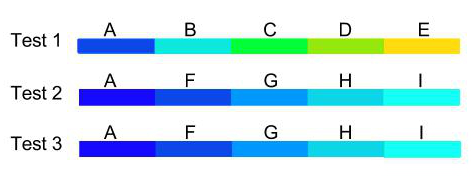
\includegraphics[width=6cm,height=3cm]{spectra.png}
\caption{A figurative spectra where each colour represents different method execution details. We see similarities between Test 2 and 3. In contrast, Test 1 is different from 2 and 3. }
\label{fig:spectra}
\end{figure}

\DIFdelbegin \DIFdel{It }\DIFdelend \DIFaddbegin \DIFadd{Once the tests are identified as being redundant, they may be removed, however it }\DIFaddend is important to understand the dangers of removing test cases. Unless two test cases are exactly the same, it is difficult to guarantee that they are redundant, even if one subsumes another. \DIFdelbegin \DIFdel{Therefore the aim }\DIFdelend \DIFaddbegin \DIFadd{This creates the need to be able to use different techniques, dependent on the project. Therefore to expand on the goal }\DIFaddend of the project\DIFdelbegin \DIFdel{is to create a framework that gives }\DIFdelend \DIFaddbegin \DIFadd{, the developed tool should give }\DIFaddend developers different approaches \DIFdelbegin \DIFdel{in }\DIFdelend \DIFaddbegin \DIFadd{for }\DIFaddend identifying redundant test cases. The \DIFdelbegin \DIFdel{framework }\DIFdelend \DIFaddbegin \DIFadd{tool }\DIFaddend should allow a developer to configure different analysis metrics and view the results \DIFdelbegin \DIFdel{through an output file. This means that the framework }\DIFdelend \DIFaddbegin \DIFadd{in a file. Overall, the tool }\DIFaddend is useful for gaining an overview and understanding of the condition of the \DIFdelbegin \DIFdel{current }\DIFdelend test suite, allowing for manual inspection to determine if \DIFdelbegin \DIFdel{potentially redundant tests are actually redundant}\DIFdelend \DIFaddbegin \DIFadd{the identified redundant tests should be removed}\DIFaddend .

Another potential use case of the \DIFdelbegin \DIFdel{framework }\DIFdelend \DIFaddbegin \DIFadd{tool }\DIFaddend is to redistribute the test cases. This can be achieved \DIFdelbegin \DIFdel{through the splitting of any highly }\DIFdelend \DIFaddbegin \DIFadd{by splitting the non }\DIFaddend redundant tests into \DIFdelbegin \DIFdel{separate test suites and running the suites at different times, }\DIFdelend \DIFaddbegin \DIFadd{another test suite and running this suite in place of the original. The original test suite may be run over night when no development is occurring. This separation of tests based on redundancy allows for a testing process, for example regression testing, to occur in a timely fashion while }\DIFaddend ensuring the original bug finding ability is retained. \DIFdelbegin \DIFdel{For example, one test suite can be run during continuous integration, and the other over night.
David Pearce}\DIFdelend \DIFaddbegin \DIFadd{This is applicable to David Pearce, he }\DIFaddend is currently writing a language called Whiley\DIFdelbegin \DIFdel{, which }\DIFdelend \DIFaddbegin \DIFadd{. The language }\DIFaddend contains an extended static checking \DIFdelbegin \DIFdel{framework }\DIFdelend \DIFaddbegin \DIFadd{tool }\DIFaddend in order to eliminate run time exceptions through formal verification techniques. In the \DIFaddbegin \DIFadd{main }\DIFaddend compiler module alone, there are roughly \DIFdelbegin \DIFdel{1500 }\DIFdelend \DIFaddbegin \DIFadd{20,000 }\DIFaddend tests. Relocating a number of these tests into another suite would result in allowing \DIFdelbegin \DIFdel{David Pearce }\DIFdelend \DIFaddbegin \DIFadd{him }\DIFaddend to increase development speed due to a reduction in the time taken to run a large test suite. \DIFdelbegin \DIFdel{Frequent execution of tests }\DIFdelend \DIFaddbegin \DIFadd{Increasing the frequency of test suite execution also }\DIFaddend allows for bugs to be traced back to code changes \DIFdelbegin \DIFdel{, using a smaller suite for every few changes means it will take less time to execute. The bug finding ability is not affected due to being able to run the full suitewhen development is not being done. 
}%DIFDELCMD < 

%DIFDELCMD < %%%
\DIFdel{Other papers examining this research area identify redundant tests using statement information, our research explored throughout the report will be using method coverage. The majority of the previous studies examined bench marks with under 1}\DIFdelend \DIFaddbegin \DIFadd{easier and reduces the time spent debugging. Therefore, by redistributing the test suite}\DIFaddend , \DIFdelbegin \DIFdel{000 test cases. For bench marks with over 1, 000 cases storing every statement execution could be costly. Therefore it would be intriguing to see to what extent can method execution data identify redundant test cases. One of the issues that previous studies reported were high level of false positive. Method execution data gives a few different ways to explore this issue which are explored in Section \ref{S:metrics}.
The aim of the paper }\DIFdelend \DIFaddbegin \DIFadd{not only does the time taken to run a test suite decrease, there is incentive for developers to execute the suite more often and in turn helping them reduce time taken to debug.
}

\DIFadd{The contributions of the report }\DIFaddend is split into two sections: 

\begin{itemize}
\item Create a \DIFdelbegin \DIFdel{framework to identify }\DIFdelend \DIFaddbegin \DIFadd{tool for identifying }\DIFaddend redundant test cases
\item Analyse different strategies \DIFdelbegin \DIFdel{to identify }\DIFdelend \DIFaddbegin \DIFadd{for identifying }\DIFaddend redundant test cases through experimenting on realistic benchmarks
\end{itemize}

\DIFdelbegin %DIFDELCMD < \newpage 
%DIFDELCMD <  \newpage %%%
\chapter{\DIFdel{Background}}%DIFAUXCMD
\addtocounter{chapter}{-1}%DIFAUXCMD
%DIFDELCMD < \label{C:related}
%DIFDELCMD < %%%
\DIFdelend \DIFaddbegin \section{\DIFadd{Outline}}
\DIFaddend 

\DIFdelbegin \section{\DIFdel{Tracing}}
%DIFAUXCMD
\addtocounter{section}{-1}%DIFAUXCMD
%DIFDELCMD < 

%DIFDELCMD < %%%
\DIFdel{There were two considered tracing frameworks to use. Implementation details of these frameworks are further discussed in Section \ref{C:workdone}.
}%DIFDELCMD < 

%DIFDELCMD < %%%
\DIFdel{The first framework considered was AspectJ. It uses byte code weaving to trace method executions; this is when a piece of code is added to existing code without modifying the code itself and can be achieved through several different ways. }%DIFDELCMD < 

%DIFDELCMD < \begin{itemize}
%DIFDELCMD < \item %%%
\DIFdel{Compile time:
The classes are compiled with the aspect weaved into them. When the jar is executed, the methods have the byte code from the aspect weaved into it already. This requires the source to be compiled with AspectJ's compiler.
}%DIFDELCMD < \item %%%
\DIFdel{Load time:
This involves binary weaving deferred until the point in which a class loader will attempt to load in a class file. This is achieved by using a command line argument notifying java to use the AspectJ class loader.
}%DIFDELCMD < \end{itemize}
%DIFDELCMD < 

%DIFDELCMD < %%%
\DIFdel{To distinguish what code to weave, and where in the existing code to weave it, a point cut can describe these in AspectJ \mbox{%DIFAUXCMD
\cite{aspectwiki}
}%DIFAUXCMD
. The other framework is Java Debugging Interface (JDI). JDI is similar to using an observer pattern. The list of classes to observe are selected, when a method is called the listening class will be notified if it has registered to be observed and will be given the information of the method call. }%DIFDELCMD < 

%DIFDELCMD < %%%
\section{\DIFdel{Performance Evaluation}}
%DIFAUXCMD
\addtocounter{section}{-1}%DIFAUXCMD
%DIFDELCMD < \label{performanceEvalBG}
%DIFDELCMD < %%%
\DIFdel{The purpose for evaluating a performance of a given application is to create an understanding of the typical performance. For this typical performance to be valid, it has to be rigorous in }\DIFdelend \DIFaddbegin \DIFadd{The report is structured as follows. Chapter 2 discusses background information that explores concepts needed to understand the following chapters as well as previous research in this area of interest. The }\DIFaddend design and implementation \DIFdelbegin \DIFdel{. This involves taking into consider a variety of factors that will be examined in reference to research papers that explore the issues.
}%DIFDELCMD < 

%DIFDELCMD < %%%
\DIFdel{Andy Georges et al. \mbox{%DIFAUXCMD
\cite{georges2007statistically}
}%DIFAUXCMD
and Steve Blackburn et al. \mbox{%DIFAUXCMD
\cite{blackburn2008wake}
}%DIFAUXCMD
present issues and alternatives to the current java performance methodologies used in research papers. They note that in premier conferences, 16 of the 50 papers examined did not examine the methodology they used. This limits the validity of the results and creates a situation where the experiment can not be reproduced. One of the main issues identified is specifying singular numbers, without expressing what the number is referring to (average, median, best, worst), leading to potential misleading representation of the results. A set of parameters that are of interest are explored in the paper, these include, heap size, start up performance, number of virtual machine (VM) invocations and handling of garbage collection. An experiment should also take into consideration the environment that the analysis is executed on.
}%DIFDELCMD < \begin{itemize}
%DIFDELCMD < \item %%%
\DIFdel{Heap Size -- A change in heap size can impact the garbage collection process. The smaller the heap size, }\DIFdelend \DIFaddbegin \DIFadd{of the tool is then examined in Chapter 3. After the tool is discussed, Chapter 4 investigates the different techniques explored and conducts and analyses experiments. Finally, Chapter 5 concludes the report and identifies future work. }\newpage 
 \newpage \chapter{\DIFadd{Background}}\label{C:related}

\DIFadd{This chapter firstly explores the current research conducted in this area, it then covers the key ideas that are needed to understand the remainder of }\DIFaddend the \DIFdelbegin \DIFdel{more often the garbage collector is run. }%DIFDELCMD < \item %%%
\DIFdel{Start Up Costs  }\DIFdelend \DIFaddbegin \DIFadd{report. These ideas are }\DIFaddend -- \DIFdelbegin \DIFdel{The costs associated with starting the application up. This will always involve class loading and just in time (JIT) re(compilation), it can also involve reading from a database and setting the application up.
}%DIFDELCMD < \item %%%
\DIFdel{Number of VM invocations -- The number of application runs that a single VM instance will execute.
}%DIFDELCMD < \item %%%
\DIFdel{Garbage Collection -- The process in identifying and removing objects that are no longer referenced.
}%DIFDELCMD < \item %%%
\DIFdel{Environment -- The hardware that the application is being run on.
}%DIFDELCMD < \end{itemize}
%DIFDELCMD < 

%DIFDELCMD < %%%
\section{\DIFdel{Grid Computing}}
%DIFAUXCMD
\addtocounter{section}{-1}%DIFAUXCMD
\DIFdel{A grid computing system is a distributed system that has no interactive work loads between machines. No interactions results in task independence being a necessity. The particular grid system used for this paper is located around Victoria University of Wellington. The machines in the grid are idle machines around the School of Engineering and Computer Science. There are a limited number of machines, therefore a total of 150 jobs can be run at a given time. Since the grid is located around an active community, if a user logs on while a process is being conducted, the application is paused until the machine returns to an idle state}\DIFdelend \DIFaddbegin \DIFadd{approaches to storing method coverage, edit distance metrics, evaluating performance of Java programs and the use of grid computing}\DIFaddend .

\section{Related Work}
\label{relatedworkRef}
\DIFaddbegin \subsection{\DIFadd{Identifying Redudant Tests}}
\DIFaddend Testing is a critical part to any software engineering process, not only to stop incidents stemming from the the product, but also partially related to the increase in popularity of agile methodologies \cite{chaos}. Many of these methodologies employ test driven development and continuous integration resulting in testing becoming more important throughout the development process. For these reasons there have been research papers that examine the different approaches that can be taken to identify redundant test cases and reduce the size of test suites \cite{wong1995effect, wong1999test, rothermel1998empirical, rothermel2002empirical,koochakzadeh2009test,zhang2011empirical,li2008static}.

\DIFdelbegin \DIFdel{It is unclear whether }\DIFdelend \DIFaddbegin \DIFadd{Whether }\DIFaddend programmatically reducing a test suite's size is worth the trade off in the ability to locate bugs \DIFaddbegin \DIFadd{is unclear}\DIFaddend .  Wong et al. \cite{wong1995effect, wong1999test} \DIFaddbegin \DIFadd{explored the impact that reducing the size of the test suite based off of code coverage had on the fault detection capability. By introducing faults into several programs and comparing the performance between the original and reduced test suites, they }\DIFaddend found that test suite reduction does not severely impact fault detection capability. In contrast to this finding, Rothermel et al. \cite{rothermel1998empirical, rothermel2002empirical} \DIFaddbegin \DIFadd{further expanded on Wong's work by using different benchmark's and performance metrics. They }\DIFaddend found that test-suite reduction can severely impact the fault detection capability. The uncertainty created by these conflicting studies motivates our research to decouple the removal of tests from the framework and move the responsibility onto \DIFdelbegin \DIFdel{the }\DIFdelend developers. 

A popular technique used in detecting redundancy involves analysing the statement executions, known as coverage information. Maurer, Garousi and Koochakzadeh \cite{koochakzadeh2009test} attempt to answer the question, is coverage information enough to determine redundant test cases? They state a redundant test case as being one that does not improve a specific criteria. For example, \DIFdelbegin \DIFdel{in Figure \ref{fig:venndiagram} we see that according to the statement coverage data of test cases , }\DIFdelend \DIFaddbegin \DIFadd{Figure \ref{fig:venndiagram} represents the statement criteria data from test cases }\DIFaddend T1 \DIFdelbegin \DIFdel{... }\DIFdelend \DIFaddbegin \DIFadd{to }\DIFaddend T5\DIFdelbegin \DIFdel{, }\DIFdelend \DIFaddbegin \DIFadd{. The figure shows that }\DIFaddend T4 and T5 are fully redundant as T3 covers the statements that are executed by \DIFdelbegin \DIFdel{those tests. They }\DIFdelend \DIFaddbegin \DIFadd{the tests. The authors }\DIFaddend looked at two other criteria, branch coverage and granularities. Granularity criteria involved splitting the tests into setup, exercise (execution), verify (assert) and lastly teardown then performing analysis over each section. They implemented two different metrics in which both used the criteria described above. The first metric examined each individual test with respect to every other test. It was calculated by measuring the percentage of a test case that is also a subset of the other test case. The second metric examined each test case with respect to every test suite as a whole. It was calculated by measuring the percentage of a test case that is covered by the test suite without the test in it. \DIFdelbegin \DIFdel{Comparing }\DIFdelend \DIFaddbegin \DIFadd{By comparing }\DIFaddend with manual inspection, they were able to determine the level of false positive and actual redundant tests. Of the redundant tests manually identified, the algorithm matched 95\% of those. However, of the tests that were manually identified as being non-redundant, 52\% of these were identified as being redundant by the algorithm. They concluded that coverage-based information is vulnerable in giving false-positives when identifying redundant test cases, suggesting common code paths as being a root cause. Statement coverage criteria gave a high rate of detection, but the implementation allowed for false positives to impact the results. 

\begin{figure}[h]
\begin{center}
\DIFdelbeginFL %DIFDELCMD < 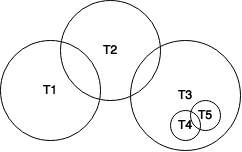
\includegraphics[]{VennDiagram.png}
%DIFDELCMD < %%%
\DIFdelendFL \DIFaddbeginFL 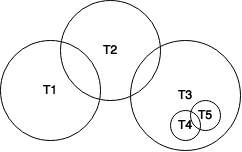
\includegraphics[width=10cm, height=6cm]{VennDiagram.png}
\DIFaddendFL \end{center}
\caption{The coverage of each test is shown by a circle. It shows that T4 and T5 are redundant as T3 already covers those statements.}
\label{fig:venndiagram}
\end{figure}

Zhang, Marinov, Zhang and Khurshid \cite{zhang2011empirical} examined the use of a greedy technique in comparison to heuristics. This required a criteria to be set by the tester, for example, statement coverage. The greedy technique would greedily select a test case that satisfies the maximum number of unsatisfied test requirements and would continue until all the test requirements had been satisfied. So the new test suite will contain exactly the same coverage as the old test suite while removing redundant test cases. This means that if a test subsumed another, then it would always be removed. The heuristic implementation was first conceived by Harrold, Gupta and Soffa \cite{harrold1993methodology} where essential test cases are selected as early as possible. Essential being that only one test case satisfies a test requirement exclusively. The heuristic approach resulted in the most cost-effective reduction, this being the amount of reduction and the fault-detection capability of the reduced test suites, showing that although greedy approach worked, there were better techniques available.

In situations where it is not possible to generate a spectrum to analyse, static analysis can be used to determine the level of redundancy. Robinson, Li and Francis \cite{li2008static} examine this. The tests for the benchmark they use are written in a high level automation framework and consist of a list of commands. The commands perform actions such as file copying and loading configurations. To identify redundant test cases they examine the test \DIFdelbegin \DIFdel{cases }\DIFdelend \DIFaddbegin \DIFadd{case }\DIFaddend commands as well as the instructions within the procedures that the test case loads. To calculate the similarities between two test cases, they consider three different metrics, Manhattan distance, unigram cosine similarity and bigram cosine similarity. They each were measuring how closely related two tests were based on the sequence of commands and procedures loaded. Their findings were similar to Maurer et al. \cite{koochakzadeh2009test} in that there are a large number of false positives. \DIFdelbegin %DIFDELCMD < 

%DIFDELCMD < %%%
\DIFdelend Static checking has several limitations in comparison to dynamic. \DIFdelbegin \DIFdel{Firstly, during }\DIFdelend \DIFaddbegin \DIFadd{The main disadvantage is the availability of data. During }\DIFaddend run-time is when a large \DIFdelbegin \DIFdel{part }\DIFdelend \DIFaddbegin \DIFadd{portion }\DIFaddend of the data trail is \DIFdelbegin \DIFdel{accessible. Before then the only information available is the method calls. }%DIFDELCMD < \todo{Talk to Dave} %%%
\DIFdel{Static checking therefore }\DIFdelend \DIFaddbegin \DIFadd{available and is important when needing to know the exact method calls and parameters passed to these methods. Static checking }\DIFaddend would provide useful information in a framework where dynamic data can not be collected\DIFdelbegin \DIFdel{and allows for the test cases to be }\DIFdelend \DIFaddbegin \DIFadd{. The framework would also need to be applicable to being }\DIFaddend examined in a static fashion such as the one used by Robinson, Li and Francis \cite{li2008static}.
\DIFdelbegin \DIFdel{Dynamic allows for more data to be collected such as the parameters passed to a method as well as the ability to be executed on more suites. The papers examined looked at the }\DIFdelend \DIFaddbegin 

\DIFadd{Taking into the related work discussed, each paper used the }\DIFaddend coverage of a test suite at several different criterion levels but none looked at the \DIFdelbegin \DIFdel{spectra }\DIFdelend \DIFaddbegin \DIFadd{method execution }\DIFaddend explicitly. This leaves a potentially useful approach to the problem that may help determine the level of redundancy within a test suite. 
\DIFdelbegin %DIFDELCMD < 

%DIFDELCMD < %%%
\DIFdelend \DIFaddbegin \subsection{\DIFadd{Calling Context}}
\DIFaddend When methods execute there is a trail of data that is left behind. Piecing together this data can show the relationships between methods, this relationship is known as a \DIFdelbegin \DIFdel{call graph}\DIFdelend \DIFaddbegin \textit{\DIFadd{call graph}}\DIFaddend . The call graph can be retrieved statically or dynamically \cite{graham1982gprof}. A static graph represents every possible run of the program. A dynamic graph represents one particular run. \DIFdelbegin \DIFdel{In contrast}\DIFdelend \DIFaddbegin \DIFadd{Comparing them}\DIFaddend , a static graph requires more information to be held and in the particular case of profiling test cases, dynamic would be more suitable due to the nature of a test case being the same for every run. Another advantage of a dynamic graph is the ability to collect functional parameters. Xiaotong Zhuang and et al. \cite{Zhuang06accurate} describe a call tree as the overall tree of every method execution. To store the full call tree would involve an excess of memory, therefore they discuss the use of a calling context tree. This tree represents the same method executions however is compressed where the edge between the nodes contains a weighting, the weighting \DIFaddbegin \DIFadd{being }\DIFaddend the number of occurrences of that method execution (calling frequency). Examining Figure \ref{fig:callgraph} shows the different variations that can be observed with the same data. The top left hand picture shows the method execution trail, where A calls B, then B calls D twice and A calls C, then C calls D once. The call graph image (top right) condenses the information into one node per method call. This method is the most condensed variation, but gives the least amount of information. Directly below this, \DIFdelbegin \DIFdel{(}\DIFdelend \DIFaddbegin \DIFadd{the }\DIFaddend calling context tree \DIFdelbegin \DIFdel{) condense }\DIFdelend \DIFaddbegin \DIFadd{condenses }\DIFaddend it slightly less. It separates each path into its own branch when it is unique to the tree, the connection between nodes contains a weighting which represent the frequency. Finally, the bottom left (call tree) creates a new path for every new method execution regardless of the uniqueness, giving us the most information about the context if the order is retained.

\begin{figure}[h]
\begin{center}
\includegraphics[width = \textwidth]{CallGraph.png}
\end{center}
\caption{A diagram showing the three different variations of Call Graph information. Where  each have a varying level of information that is stored.}
\label{fig:callgraph}
\end{figure}

\DIFaddbegin \subsection{\DIFadd{Edit Distance Metrics}}
\label{editdistbg}
\DIFaddend Edit distance algorithms play an important part in many domains, ranging from signal processing to mutations in genome sequences \cite{navarro2001guided}. It calculates the number of edit operations needed to go from one string to another\DIFaddbegin \DIFadd{, in our research they are used to calculate the difference between test case spectras}\DIFaddend . There are a variety of different implementations of edit distance metrics. Cohen, Ravikumar and Fienberg \cite{cohen2003comparison} explore different edit distance metrics for name matching. They concluded that Monge and Elkan \cite{monge1997efficient} performed the best for string edit-distance metrics. The metric works by splitting the two strings into tokens, \DIFdelbegin \DIFdel{these }\DIFdelend \DIFaddbegin \DIFadd{the best matching }\DIFaddend tokens are then calculated to find the similarity using other common metrics such as Levenshtein distance. One of the other techniques they explored was the Levenshtein distance \cite{levenshtein1966binary} metric by itself. This metric is the minimal number of operations that can be done to make one \DIFdelbegin \DIFdel{tests }\DIFdelend \DIFaddbegin \DIFadd{test's }\DIFaddend spectrum equal to another. These operations are inserting, deleting or substituting and a cost is associated with completing an operation. The maximum difference is the size of the larger \DIFdelbegin \DIFdel{of the two spectra's}\DIFdelend \DIFaddbegin \DIFadd{spectra}\DIFaddend . The amount of redundancy is calculated by dividing the cost of operations with the max difference in order to normalize the value. This value \DIFdelbegin \DIFdel{will be }\DIFdelend \DIFaddbegin \DIFadd{is }\DIFaddend the percentage of \DIFdelbegin \DIFdel{tests that are }\DIFdelend \DIFaddbegin \DIFadd{the test that is }\DIFaddend not redundant, \DIFdelbegin \DIFdel{we minus this value by }\DIFdelend \DIFaddbegin \DIFadd{the value }\DIFaddend 1 \DIFaddbegin \DIFadd{is then subtracted by the value }\DIFaddend to give the redundant percentage.

\DIFaddbegin \DIFadd{An example of Levenshtein is shown in Table \ref{levenTable}, where 'kitchen' is being changed into 'kitten'. The example shows the number of operations needed is 2, and the max potential needed if the two strings were completely different is 7, as kitchen contains 7 characters. The redundancy is calculated by subtracting 1 from the cost over the max potential cost $(1 - (2/7)) $. The outcome being that the words contain 71\% redundant information. 
}

\begin{table}[H]
\centering

\begin{tabular}{|l|l|l|}
\hline
{\bf \DIFaddFL{Previous State}} & {\bf \DIFaddFL{Current State}} & {\bf \DIFaddFL{Operation}}                      \\ \hline
\DIFaddFL{-                    }& \DIFaddFL{kitten              }& \DIFaddFL{-                                    }\\ \hline
\DIFaddFL{kitten               }& \DIFaddFL{kitcen              }& \DIFaddFL{Substitution of `t' with `c'         }\\ \hline
\DIFaddFL{kitcen               }& \DIFaddFL{kitchen             }& \DIFaddFL{Insertion of `h' between `c' and `e' }\\ \hline
\end{tabular}
\caption{\DIFaddFL{Using Levenshtein edit distance metric to transform kitten to kitchen.}}
\label{levenTable}
\end{table}

\DIFadd{An example of Monge }\& \DIFadd{Elkan is shown in Table \ref{mongeTable}. The comparison of the strings `paul johnson' and `johson paule' are being compared. Each of the strings get broken down into two tokens and the best matches are identified and used for the final score. The table shows that the final score of the Monge }\& \DIFadd{Elkan is taking into account `paul' }\& \DIFadd{`paule' and `johnson' }\& \DIFadd{`johson'. Using these two matches, the final result is 1/2 * (.85 + .80) = 0.825.
}

\begin{table}[H]
\centering

\begin{tabular}{|l|l|}
\hline
\textbf{\DIFaddFL{Input string 1:}}        & \DIFaddFL{paul johnson }\\ \hline
\textbf{\DIFaddFL{Input string 2:}}        & \DIFaddFL{johson paule }\\ \hline
                                &              \\ \hline
\DIFaddFL{Levenshtein("paul","johson")    }& \DIFaddFL{0.00         }\\ \hline
\DIFaddFL{Levenshtein("paul","paule")     }& \DIFaddFL{0.80         }\\ \hline
\DIFaddFL{Levenshtein("johnson","paule")  }& \DIFaddFL{0.00         }\\ \hline
\DIFaddFL{Levenshtein("johnson","johson") }& \DIFaddFL{0.85         }\\ \hline
\end{tabular}
\caption{\DIFaddFL{The Monge }\& \DIFaddFL{Elkan edit distance metric to calculate the similarity between "paul johnson" and "johson paule"}}
\label{mongeTable}
\end{table}



\subsection{\DIFadd{Wilcoxon Signed Rank Test}}

\DIFaddend A Wilcoxon Signed Rank test is used to infer whether there are any significant differences between the techniques implemented in this \DIFdelbegin \DIFdel{paper}\DIFdelend \DIFaddbegin \DIFadd{report}\DIFaddend . The Wilcoxon Signed Rank test was first proposed by Frank Wilcoxon in 1945 \cite{wilcoxon1945individual}. It is a nonparametric test for comparing two pair groups. A nonparametric test is a collective term that \DIFdelbegin \DIFdel{are }\DIFdelend \DIFaddbegin \DIFadd{is }\DIFaddend given to inferences that are valid under less confining assumptions than classical statistical inferences \cite{nonparametric}. The test does not assume that the data follows a normal distribution which is ideal for the data presented in our research and is used when two nominal variables and one measure variable is being measured \cite{mcdonald2009handbook}.
\DIFdelbegin %DIFDELCMD < \newpage 
%DIFDELCMD <  \newpage %%%
\chapter{\DIFdel{Design and Implementation}}%DIFAUXCMD
\addtocounter{chapter}{-1}%DIFAUXCMD
%DIFDELCMD < \label{C:workdone}
%DIFDELCMD < %%%
\DIFdelend 

\section{\DIFdelbegin \DIFdel{Overview}\DIFdelend \DIFaddbegin \DIFadd{Performance Evaluation}\DIFaddend }
\DIFdelbegin %DIFDELCMD < 

%DIFDELCMD < \todo{REDO ONCE FINISHED SECTION}
%DIFDELCMD < 

%DIFDELCMD < %%%
\section{\DIFdel{Tool}}
%DIFAUXCMD
\addtocounter{section}{-1}%DIFAUXCMD
%DIFDELCMD < \label{S:framework}
%DIFDELCMD < %%%
\DIFdel{An aim of the project as mentioned in Section \ref{C:intro} is to create a tool to allow developers to }\DIFdelend \DIFaddbegin \label{performanceEvalBG}
\DIFadd{Throughout the report different techniques are designed and implemented to }\DIFaddend identify redundant test cases. \DIFdelbegin \DIFdel{The tool consists of a variation of settings that give developers a range of options when deciding the different confidence levels they are wanting. The tool allows for }\DIFdelend \DIFaddbegin \DIFadd{To evaluate the techniques, experiments are conducted and must cohere to a standard procedure. The purpose for evaluating the performance of a given technique is to create an understanding of }\DIFaddend the \DIFdelbegin \DIFdel{developers to firstly trace the test suite of an application. This data is then analysed to produce a list of redundant test cases. To get the tool into a usable state, several impediments had to be overcome and are discussed in the following section.
}%DIFDELCMD < \todo{@DJ. Should i give overview of them here?}
%DIFDELCMD < %%%
\DIFdelend \DIFaddbegin \DIFadd{typical performance. For this typical performance to be valid, it has to be rigorous in design and implementation. This involves taking into consideration a variety of factors that will be examined in reference to research papers that explore the issues.
}\DIFaddend 

\DIFdelbegin \subsection{\DIFdel{Pipeline}}
%DIFAUXCMD
\addtocounter{subsection}{-1}%DIFAUXCMD
\DIFdel{The first issue encountered is the time taken to analyse the data. To conduct the analysis, every test is compared to every other test. The issue arises when the spectrum's of the test cases contain tens of thousands of method calls. This results in the analysis taking up to several days to complete. The approach identified to reduce the time is a pipeline combined with time reduction strategies. }%DIFDELCMD < 

%DIFDELCMD < %%%
\DIFdel{The pipeline approach is shown in Figure \ref{fig:pipeline}. The idea is to use analysis stages to reduce the number of comparisons each additional stage has to compute. Each analysis stage can be set by the developer within a properties file, these settings are }\DIFdelend \DIFaddbegin \DIFadd{Andy Georges et al. \mbox{%DIFAUXCMD
\cite{georges2007statistically}
}%DIFAUXCMD
and Steve Blackburn et al. \mbox{%DIFAUXCMD
\cite{blackburn2008wake}
}%DIFAUXCMD
present issues and alternatives to the current Java performance methodologies used in research papers. They note that in premier conferences, 16 of the 50 papers examined did not discuss the methodology they used. This limits the validity of the results and creates a situation where the experiment cannot be reproduced. One of the main issues identified is specifying singular numbers, without expressing what the number is referring to (average, median, best, worst). This leads to a misleading representation of the results. A set of parameters that are of interest are explored in the paper, these include, heap size, start up performance, number of virtual machine (VM) invocations and handling of garbage collection. An experiment should also take into consideration the environment that the analysis is executed on:
}\begin{itemize}
\item \textbf{\DIFadd{Heap Size}} \DIFaddend -- \DIFdelbegin \DIFdel{the spectra type, analysis metric to use and level of redundancy for each. There are two approaches that can be used to reduce the time taken to analyse the data }\DIFdelend \DIFaddbegin \DIFadd{A change in heap size can impact the garbage collection process. The smaller the heap size, the more often the garbage collector is run.
}\item \textbf{\DIFadd{Start Up Costs}}  \DIFaddend -- \DIFdelbegin \DIFdel{use of a heuristic and concurrent execution.
}\DIFdelend \DIFaddbegin \DIFadd{The costs associated with starting the application up. This will always involve class loading and just in time (JIT) re(compilation), it can also involve reading from a database and setting the application up.
}\item \textbf{\DIFadd{Number of VM invocations}} \DIFadd{-- The number of application runs that a single VM instance will execute.
}\item \textbf{\DIFadd{Garbage Collection}} \DIFadd{-- The process in identifying and removing objects that are no longer referenced.
}\item \textbf{\DIFadd{Environment}} \DIFadd{-- The hardware that the application is being run on.
}\end{itemize}
\DIFaddend 

\DIFdelbegin %DIFDELCMD < \begin{figure}[h]
%DIFDELCMD < 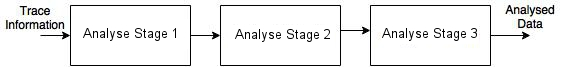
\includegraphics[width=\textwidth]{Pipeline.jpg}
%DIFDELCMD < %%%
%DIFDELCMD < \caption{%
{%DIFAUXCMD
\DIFdel{Trace information goes in at the start of the pipeline. After each stage there will be a reduction of comparisons that the next stage has to complete. The last stages should be the most computationally heavy.}}
%DIFAUXCMD
%DIFDELCMD < \label{fig:pipeline}
%DIFDELCMD < \end{figure}
%DIFDELCMD < 

%DIFDELCMD < %%%
\subsection{\DIFdel{Time reduction}}
%DIFAUXCMD
\addtocounter{subsection}{-1}%DIFAUXCMD
%DIFDELCMD < 

%DIFDELCMD < %%%
\subsubsection{\DIFdel{Heuristic}}
%DIFAUXCMD
\addtocounter{subsubsection}{-1}%DIFAUXCMD
\DIFdel{The heuristic examined a subset of }\DIFdelend \DIFaddbegin \section{\DIFadd{Grid Computing}}
\DIFadd{The time intensive nature of conducting the experiments resulted in a single computer not being adequate. A grid computing system was used instead, it is a distributed system of multiple machines that have no interactive tasks between each other. No interactions results in task independence being a necessity. The particular grid system used for this report is located at Victoria University of Wellington. The machines in }\DIFaddend the \DIFdelbegin \DIFdel{available data. A subset of data created a trade off between confidence and speed. Increasing the confidence allows us to increase the speed. The following illustrates an example of this .
}\paragraph{}
%DIFAUXCMD
\addtocounter{paragraph}{-1}%DIFAUXCMD
\DIFdel{$K,I,T,C,H,E,N \neq K,I,T,E,N,Z $
}\paragraph{}
%DIFAUXCMD
\addtocounter{paragraph}{-1}%DIFAUXCMD
\DIFdel{In this case, the two test cases would not be redundant due to them having a large difference in method calls.
}\paragraph{}
%DIFAUXCMD
\addtocounter{paragraph}{-1}%DIFAUXCMD
\DIFdel{$K,I,T,C,H,E,N \approx K,I,T,C,H,N$
}\paragraph{}
%DIFAUXCMD
\addtocounter{paragraph}{-1}%DIFAUXCMD
\DIFdel{There is a chance that these two may be redundant so it implies it should be get through the analysing stage onto the next. Using a benchmark example of Whiley on the wyc package, a heuristic approach enables us to decrease the number of comparisons from 90, 902 to 38 for the most computationally heavy stage. }\DIFdelend \DIFaddbegin \DIFadd{grid are idle machines around the School of Engineering and Computer Science. There are a limited number of machines, therefore a total of 150 jobs can be run at a given time. Since the grid is located around an active community, if a user logs on while a process is being conducted, the application is paused until the machine returns to an idle state. }\newpage 
 \newpage \chapter{\DIFadd{Design and Implementation}}\label{C:workdone}
\DIFaddend 

\DIFdelbegin \subsubsection{\DIFdel{Concurrent}}
%DIFAUXCMD
\addtocounter{subsubsection}{-1}%DIFAUXCMD
\DIFdelend \DIFaddbegin \section{\DIFadd{Overview}}
\DIFaddend 

\DIFdelbegin \DIFdel{Concurrent execution was implemented by splitting the test cases up into 8 different parts, each part knew the test cases that it had to compare. A new thread executed each split, making the implementation relatively easy. The concurrent execution lead to a decrease in roughly 2 times the time taken to analyse  but lead to a trade off in increased memory usage. This meant concurrent execution was only usable for the smaller bench marks. }\DIFdelend \DIFaddbegin \DIFadd{The goal of the project as mentioned in Section \ref{C:intro} is to create a tool to allow developers to identify redundant test cases. The tool can be split into several different sections and each section will be discussed in this chapter. The first objective of the tool was to trace the test data. This involved exploring two different frameworks and comparing the usability of each. After the tool was able to trace the data, we had to determine what spectras we were interested in. The three different spectra types are then discussed. The data that was traced from each test case was then compared to each other to determine the level of redundancy between each test using edit distance metrics. Throughout the testing of the tool, one of the main impediments was the time taken to analysis the large amount of data. We examine how pipelining the output of a heuristic analysis into more computationally heavy analysis decreases the time taken. The final two sections discuss two more advanced areas of the tool. Firstly, retrieving the parameters of the method calls and discussing the trade off parameters create between time taken and more information to analyse. Secondly, giving a weighting to each method call was implemented with the purpose of reducing false positives.
}\DIFaddend 

\DIFdelbegin \subsection{\DIFdel{Saving to the Network}}
%DIFAUXCMD
\addtocounter{subsection}{-1}%DIFAUXCMD
\DIFdel{Saving the data to network solved two issues. Firstly, it allowed for the datato be reanalysed without having to execute the test suite again. Secondly, the test data had to be accessible to the grid machines. Saving the data on my user profile allowed for the data to be retrieved, regardless of the machine an analysing job was being run on. }%DIFDELCMD < 

%DIFDELCMD < %%%
\DIFdelend \section{Tracing}
\label{S:trace}
\DIFdelbegin \DIFdel{During the test suite execution, each test case creates a data trail that is partially recorded. Accessing different sections of the data trail gives different information . }%DIFDELCMD < \todo{Hmmmmm}
%DIFDELCMD < 

%DIFDELCMD < %%%
\DIFdelend \DIFaddbegin \DIFadd{A fundamental requirement for this project was to trace which methods were executed by a test. As }\DIFaddend David Pearce's language Whiley is written in Java\DIFdelbegin \DIFdel{. Taking this into account }\DIFdelend \DIFaddbegin \DIFadd{, }\DIFaddend it was decided to use Java to trace a \DIFdelbegin \DIFdel{tests spectrum. There are two viable options, the Java }\DIFdelend \DIFaddbegin \DIFadd{test. There were two considered tracing frameworks. The first framework considered was AspectJ. The technique that AspectJ uses is called Aspect Oriented Programming (AOP). AOP can be used to add code to an existing program without modifying the source code, this code added is known as an aspect. This process be achieved through the following methods:
}

\begin{itemize}
\item \textbf{\DIFadd{Compile time}} \DIFadd{--
The classes are compiled with the aspect woven into them. When the program is executed, the methods have the code from the aspect woven into it already. This requires the source to be compiled with AspectJ's compiler.
}\item \textbf{\DIFadd{Load time}} \DIFadd{--
The weaving process is deferred until the point at which a class loader attempts to load in a class file. Load time modification is achieved by using a command line argument notifying Java to use the AspectJ class loader.
}\end{itemize}

\DIFadd{To distinguish what code to weave, and where in the existing code to weave it, a point cut can describe these in AspectJ \mbox{%DIFAUXCMD
\cite{aspectj}
}%DIFAUXCMD
. The other framework we considered was the Java }\DIFaddend Debugging Interface (JDI)\DIFdelbegin \DIFdel{or AspectJ, as discussed in Section \ref{C:related}}\DIFdelend \DIFaddbegin \DIFadd{. JDI is similar to using an observer pattern. The list of classes to observe are selected, when a method is called the listening class will be notified if the method has registered to be observed and will be given the information about the method call}\DIFaddend . 

It was decided to use AspectJ over JDI. AspectJ \DIFdelbegin \DIFdel{is }\DIFdelend \DIFaddbegin \DIFadd{was }\DIFaddend easier to choose which methods to record and returns the actual object when retrieving the parameters of the method call\DIFdelbegin \DIFdel{allowing for reflection to be used to retrieve the information for every object. }\DIFdelend \DIFaddbegin \DIFadd{. This detail becomes important when we explore tracing parameter values in Section \ref{parameterTrace}. In comparison, }\DIFaddend JDI was faster to execute, however there was a limited amount of documentation available and the parameters returned were not the actual objects\DIFdelbegin \DIFdel{, meaning that standard reflection could not be used to retrieve the values}\DIFdelend . The decision to use AspectJ was based off this trade off between information and performance. \DIFdelbegin \DIFdel{The analysis tool was able to be altered to increase the performance of it, so having }\DIFdelend \DIFaddbegin \DIFadd{Decoupling the data gathering and data analyse in the tool removed the emphasis on retrieval performance and resulted in }\DIFaddend the extra information \DIFdelbegin \DIFdel{that AspectJ gave was more importantthan an taking less time to execute}\DIFdelend \DIFaddbegin \DIFadd{being more important}\DIFaddend .

To get AspectJ to trace the method \DIFdelbegin \DIFdel{execution}\DIFdelend \DIFaddbegin \DIFadd{details}\DIFaddend , a point cut was made to record every execution. A simplified version of the aspect is shown in Figure \ref{fig:aspectused}. There are two point cuts within the aspect, the first \DIFdelbegin \DIFdel{pointcut }\DIFdelend \DIFaddbegin \DIFadd{point cut }\DIFaddend is going to be called for every method which has a \DIFdelbegin \DIFdel{junit }\DIFdelend \DIFaddbegin \DIFadd{Junit }\DIFaddend \@Test annotation attached to it. This will then let a static service know that a new test has been started. The second \DIFdelbegin \DIFdel{pointcut }\DIFdelend \DIFaddbegin \DIFadd{point cut }\DIFaddend is used to trace everything \DIFdelbegin \DIFdel{but methods attached to }\DIFdelend \DIFaddbegin \DIFadd{apart from methods with a  }\DIFaddend \@Test annotation \DIFdelbegin \DIFdel{. 
}%DIFDELCMD < 

%DIFDELCMD < %%%
\DIFdelend \DIFaddbegin \DIFadd{attached. }\DIFaddend The next stage was to weave the \DIFdelbegin \DIFdel{point cuts }\DIFdelend \DIFaddbegin \DIFadd{aspect }\DIFaddend into the benchmark. Using compile time weaving would have meant that each benchmark needed to be recompiled using the aspect compiler. In contrast\DIFdelbegin \DIFdel{to load time , which }\DIFdelend \DIFaddbegin \DIFadd{, load time }\DIFaddend only requires the AspectJ class loader to be passed through a command line argument. \DIFdelbegin \DIFdel{The load }\DIFdelend \DIFaddbegin \DIFadd{Load }\DIFaddend time was chosen for it's ease of use when working with external benchmarks as it only required AspectJ's class loader\DIFdelbegin \DIFdel{to be use}\DIFdelend .

\DIFdelbegin \subsection{\DIFdel{Parameter Values}}
%DIFAUXCMD
\addtocounter{subsection}{-1}%DIFAUXCMD
\DIFdel{The related work in Section \ref{relatedworkRef} explored the statement coverage while ignoring the parameter values that each method was passed. It could be argued that due to knowing the statement path, parameters are irrelevant as you know the path the method will take, and parameters will not add any more information. When using method execution details alone, these become crucial when determining the level of redundancy due to the limited amount of information that the method details alone gives us. 
}%DIFDELCMD < 

%DIFDELCMD < %%%
\DIFdel{AspectJ gives direct access to the object's that are contained in the parameter values of the method. This allows for reflection to be used to retrieve the objects in a representable state. By using reflection, the fields of the objects can be retrieved and returned in a string. This string is then examined to remove any java object reference location and stored. Initially it was decided to examine primitive types only, this resulted in a very limited number of parameters and did not have the desired effect of decreasing the level of false positives while increasing the time and memory. Changing to reflection allowed for more detailed parameters to be collected. This increases the certainty about the whether two tests are redundant, decreasing the false positives but increasing the time and memory even more than the use of primitives only. 
}%DIFDELCMD < 

%DIFDELCMD < %%%
\DIFdel{The most common use case of the tool would involve the use of parameters therefore it was decided to optimize this through storing the data with parameters. The optimization involved saving the parameters with the trace information. If parameters value is set to false, the parameters have to be split off rather than added on. This means that setting the parameters to false would increase the set up time.
}%DIFDELCMD < 

%DIFDELCMD < %%%
\DIFdelend \begin{figure}[h]
\begin{center}
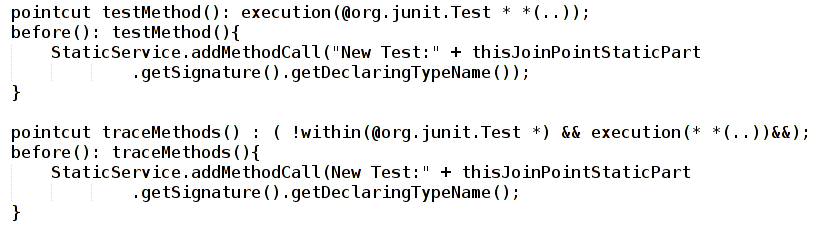
\includegraphics[width = \textwidth]{aspect.png}
\end{center}
\caption{A simplified point cut within AspectJ. The first \DIFdelbeginFL \DIFdelFL{pointcut }\DIFdelendFL \DIFaddbeginFL \DIFaddFL{point cut }\DIFaddendFL is for when a new test is executed and the second when a new method is executed.}
\label{fig:aspectused}
\end{figure}

\section{Test Spectra}
\label{S:spectra}
The idea of a spectrum was previously identified in Chapter \ref{C:intro}. Reexamining the idea, a spectrum is some abstraction of the \DIFaddbegin \DIFadd{method execution }\DIFaddend information that is retrievable during the execution of a test. \DIFdelbegin \DIFdel{Our tool is particularly interested in utilising the method execution details. This allows there to be several }\DIFdelend \DIFaddbegin \DIFadd{The data retrieved can be split into three }\DIFaddend different types of spectra\DIFdelbegin \DIFdel{. The main three spectra examined are }\DIFdelend \DIFaddbegin \DIFadd{, these are }\DIFaddend \textit{\DIFdelbegin \DIFdel{set}\DIFdelend \DIFaddbegin \DIFadd{unique method calls}\DIFaddend }, \textit{\DIFdelbegin \DIFdel{list}\DIFdelend \DIFaddbegin \DIFadd{every method call}\DIFaddend } and \textit{calling context}. To explore the different spectra's, an example trace of methods, 'kitten' will be used. Each letter represents a method execution and each letter is executed \DIFdelbegin \DIFdel{from the }%DIFDELCMD < \todo{same parent method}%%%
\DIFdelend \DIFaddbegin \DIFadd{by the same method}\DIFaddend . The different spectra's take up different levels of resources. The resources explored are -- time taken \DIFdelbegin \DIFdel{, memory and complexity}\DIFdelend \DIFaddbegin \DIFadd{and memory}\DIFaddend . 

\subsection{\DIFdelbegin \DIFdel{Set}\DIFdelend \DIFaddbegin \DIFadd{Unique Method Calls}\DIFaddend }
\DIFdelbegin \DIFdel{A set of method executions }\DIFdelend \DIFaddbegin \DIFadd{The unique method call spectra }\DIFaddend is where every method execution is only taken into account once. Examining the example trace, the output would be 'kiten', with the difference being the removal of the repeated 't' method. The implication of limiting the method calls to one per method call on the number of comparisons will be dependent the benchmark. Using Whiley Compiler benchmark as an example, there are 494 unique method executions for a single test and 80,000 method calls to these method executions. Utilising the \DIFdelbegin \DIFdel{set method }\DIFdelend \DIFaddbegin \DIFadd{unique method call method}\DIFaddend , the tool will only \DIFdelbegin \DIFdel{examine the }\DIFdelend \DIFaddbegin \DIFadd{compute the redundancy of }\DIFaddend 494 \DIFaddbegin \DIFadd{method executions}\DIFaddend , rather than the 80,000, \DIFdelbegin \DIFdel{a decrease of }\DIFdelend $\rfrac{6}{1000}$ \DIFdelbegin \DIFdel{. This leads to a substantial reduction in }\DIFdelend \DIFaddbegin \DIFadd{of the original amount. The motivation of the spectra is to substantially reduce }\DIFaddend the time taken and memory used. However, \DIFaddbegin \DIFadd{by }\DIFaddend decreasing the amount of data means that there is a decrease in confidence that the tests produced are redundant test cases. \DIFdelbegin \DIFdel{The motivation behind the spectra to use it as a heuristic pipeline, as }\DIFdelend \DIFaddbegin \DIFadd{How this fits into the tool is }\DIFaddend explored in Section \DIFdelbegin \DIFdel{\ref{S:framework}. }\DIFdelend \DIFaddbegin \DIFadd{\ref{pipelinesection}. }\todo{Unsure if this last sentance is good or just to remove}
\DIFaddend 

\subsection{\DIFdelbegin \DIFdel{List}\DIFdelend \DIFaddbegin \DIFadd{Every Method Call}\DIFaddend }
\DIFdelbegin \DIFdel{A }\DIFdelend \DIFaddbegin \DIFadd{The every method call takes into every method execution, analogous to a }\DIFaddend list of method \DIFdelbegin \DIFdel{executions is where every }\DIFdelend \DIFaddbegin \DIFadd{calls. This spectra is the same as using a calling context of one, where only the highest }\DIFaddend method execution is \DIFdelbegin \DIFdel{taken into account}\DIFdelend \DIFaddbegin \DIFadd{examined}\DIFaddend . Examining the example trace, the output would be 'kitten', with there being no difference between the two. Using the Whiley Compiler benchmark as an example, a list spectra would \DIFdelbegin \DIFdel{examine }\DIFdelend \DIFaddbegin \DIFadd{compute the redundancy of }\DIFaddend all 80,000 method calls\DIFdelbegin \DIFdel{to calculate the level of redundancy. A list spectra is the same as using a calling context of one, where only the highest method execution is examined. }\DIFdelend \DIFaddbegin \DIFadd{. }\DIFaddend Comparing this to \DIFdelbegin \DIFdel{a set }\DIFdelend \DIFaddbegin \DIFadd{the unique method call }\DIFaddend spectra, this is expected to lead to an increase in the time taken but \DIFdelbegin \DIFdel{increase the confidence of the redundancy. 
The motivation behind the approach is to use during the second stage in the pipeline to decrease the amount of comparisons that the final pipeline should do. This approach would not be used in the last pipeline as there is limited sense to use a subset of information retrieved from the test cases.
}\DIFdelend \DIFaddbegin \DIFadd{also increase the credibility of the results. 
}\DIFaddend 

\subsection{Calling Context}
A calling context \DIFdelbegin \DIFdel{of method executions is where each method call, the trace data }\DIFdelend contains a separate \DIFdelbegin %DIFDELCMD < \todo{node} %%%
\DIFdel{for each call stack }\DIFdelend \DIFaddbegin \DIFadd{node for each parent method }\DIFaddend that the method was called \DIFdelbegin \DIFdel{with \mbox{%DIFAUXCMD
\cite{callingcontext}
}%DIFAUXCMD
. The depth }\DIFdelend \DIFaddbegin \DIFadd{from \mbox{%DIFAUXCMD
\cite{Zhuang06accurate}
}%DIFAUXCMD
. The number of call retained }\DIFaddend is referred to as \DIFdelbegin \DIFdel{K. }\DIFdelend \DIFaddbegin \DIFadd{the K depth. The motivation behind the approach is to increase the credibility of the results by taking into account for more data. The consequence of increasing the amount of data is an increase in the time taken and memory used to analyse. }\DIFaddend Examining the example trace, the output would be 'Parent $\rightarrow$ k, Parent $\rightarrow$ i, Parent $\rightarrow$ t ...). Using \DIFaddbegin \DIFadd{the }\DIFaddend Whiley Compiler benchmark as an example, a calling context spectra would examine all 80,000 method calls, with each containing K depth of method calls. 
\DIFdelbegin \DIFdel{The motivation behind the approach is to be the final stage in the pipeline. Having this approach as the final pipeline would give the highest confidence that the tests were redundant, as it has access to the most information.
}\DIFdelend 

To retrieve the calling context in Java, the current stack trace of a method call is examined and then parsed to retrieve the relevant information. This parsing involves removing the method calls that are used to retrieve the stack trace and any memory location details.  \DIFaddbegin \todo{Should i remove this or introduce every section?}\DIFaddend In the next section, two different analysis metrics are introduced and examined.

\section{Analysis Metrics}
\label{S:metrics}
\DIFdelbegin %DIFDELCMD < 

%DIFDELCMD < %%%
\DIFdel{There were a variety of different edit distance metrics to consider, the two of particular interest were Monge }%DIFDELCMD < \& %%%
\DIFdel{Elkan \mbox{%DIFAUXCMD
\cite{monge1997efficient}
}%DIFAUXCMD
and Levenshtein \mbox{%DIFAUXCMD
\cite{levenshtein1966binary}
}%DIFAUXCMD
. These were explored in Chapter \ref{C:related}, it is discussed how }\DIFdelend \DIFaddbegin \DIFadd{The data retrieved from the tracing process needs to be analysed to produce a quantitative value. The value produced will be used to determine the level of similarity between two test cases. Edit distance metrics were discussed in Section \ref{editdistbg}, with two different edit distance metrics considered. They were }\DIFaddend Monge \& Elkan \DIFdelbegin \DIFdel{metric }\DIFdelend \DIFaddbegin \DIFadd{\mbox{%DIFAUXCMD
\cite{monge1997efficient}
}%DIFAUXCMD
which }\DIFaddend splits the strings into \DIFdelbegin \DIFdel{tokens }\DIFdelend \DIFaddbegin \DIFadd{sections }\DIFaddend and compares the \DIFdelbegin \DIFdel{tokens while Levenshtein looks over the whole string}\DIFdelend \DIFaddbegin \DIFadd{sections and Levenshtein \mbox{%DIFAUXCMD
\cite{levenshtein1966binary}
}%DIFAUXCMD
which compares tokens, generally tokens are single characters}\DIFaddend . 

For both of the algorithms, there were publicly available frameworks that implemented them. \DIFdelbegin \DIFdel{Monge }%DIFDELCMD < \& %%%
\DIFdel{Elkan distance metric split a method call into sections and ran Levenshtein over them. In contrast, the separate Levenshtein implementation }\DIFdelend \DIFaddbegin \DIFadd{Both implementations }\DIFaddend allowed for the method calls to be \DIFdelbegin \DIFdel{split into tokens, these tokens represented a whole method call rather than the method call being split up as in }\DIFdelend \DIFaddbegin \DIFadd{represented with a token. Each test case contained a list of the tokens to represent the trace information of it. The issue with }\DIFaddend Monge \& Elkan \DIFdelbegin \DIFdel{. Visualizing the idea }\DIFdelend \DIFaddbegin \DIFadd{was it attempted to find the best match. Attempting to find the best match would increase the time taken, perform unnecessary computation for our requirements and increase the false positive rate. Using an example of trace information }\DIFaddend in Figure \ref{fig:mongevleven}. The \DIFdelbegin \DIFdel{top figure shows Monge and Elkan would split the method calls, comparing each token to produce the number of operations at a character level. The implementation of Levenshtein allows for whole method calls as shown to be compared to each other, for instance, if one method callis different then the number of operations is one. Comparison of method calls increases the comparison speed and decreased the time taken}\DIFdelend \DIFaddbegin \DIFadd{implementation of Monge }\& \DIFadd{Elkan would find the best match, in turn matching 'Method Call' in test case 1 to the 'Method Call' in test case 2. Levenshtein did not search for a match, and instead only looked at the opposing method call. This one to one matching was preferred as we were interested in the order of the method calls as well as what methods were called}\DIFaddend . Overall, Levenshtein integrated better into \DIFdelbegin \DIFdel{our tool}\DIFdelend \DIFaddbegin \DIFadd{the tool's ability to identify redundant test cases}\DIFaddend .

\begin{figure}[h]
\begin{center}
\DIFdelbeginFL %DIFDELCMD < \includegraphics[width = \textwidth]{mongevleven.png}
%DIFDELCMD < %%%
\DIFdelendFL \DIFaddbeginFL \includegraphics[width = \textwidth]{MongeVLeven.png}
\DIFaddendFL \end{center}
\caption{An example showing how Monge \& Elkan split the method calls into token, where Levenshtein represents the method calls as a whole.}
\label{fig:mongevleven}
\end{figure}

\DIFdelbegin \DIFdel{An example is shown in Table \ref{levenTable}, where 'kitchen' is being changed into 'kitten'. The example shows the number of operations needed is 2, and the max potential needed if the two strings were completely differentis 7 as kitchen contains 7 characters. The redundancy is calculated by subtracting }\DIFdelend \DIFaddbegin \section{\DIFadd{Pipeline}}
\label{pipelinesection}
\DIFadd{For the tool to help developers reduce the number of redundant tests, it has to analysis the information within an acceptable time frame. By comparing every test with every other while using all of the available information (calling context), this resulted in the analysis taking several days to complete. This is not considered an acceptable time frame. This issue arises when the spectrum's of the test cases contain tens of thousands of method calls. A pipeline approach was implemented which utilised the unique method call spectra as a heuristic. The goal of the pipeline was that each stage should soundly eliminate pairs from consideration that the following stages would have removed. The pipeline approach is shown in Figure \ref{fig:pipeline}. Each analysis stage can be set by the developer within a properties file, these settings are -- the spectra type, analysis metric to use and level of redundancy for each.
}

\DIFadd{To further expand on the heuristic idea. Unique method calls spectra was used as it examined a subset of the available data. Inspecting the subset of data increased the speed of comparison but as a consequence decreased the credibility of our results. The following illustrates an example of this where each character represents a method call.
}\paragraph{\DIFadd{Comparison 1}}
\DIFadd{$K,I,T,C,H,E,N$ }\& \DIFadd{$K,I,B,E,N,Z $
}\paragraph{\DIFadd{Comparison 2}}
\DIFadd{$K,I,T,C,H,E,N$ }\& \DIFadd{$K,I,T,C,H,N$
}\paragraph{}
\DIFadd{Inspecting comparison }\DIFaddend 1\DIFdelbegin \DIFdel{from the cost over the max potential cost $(1 - (2/7)) $. The outcome being that the words contain 71\% redundant information }\DIFdelend \DIFaddbegin \DIFadd{, it is clear that the two sets of trace information are different. Examining comparison 2, there is a chance that the tests may be redundant so the comparison should be get through the analysing stage and onto the next. Using a benchmark example of Whiley on the wyc package, a heuristic approach enables us to decrease the number of test case comparisons from 90,902 to 100 for the most computationally heavy stage.
}

\DIFadd{The list spectra may also be used as another type of heuristic. The motivation behind the spectra is to use during the second stage in the pipeline to decrease the amount of comparisons that the final pipeline should do. This approach would not be used in the last pipeline as there is limited sense to use a subset of information retrieved from the test cases}\DIFaddend .

\DIFdelbegin %DIFDELCMD < \begin{table}[]
%DIFDELCMD < \centering
%DIFDELCMD < %%%
\DIFdelend \DIFaddbegin \begin{figure}[h]
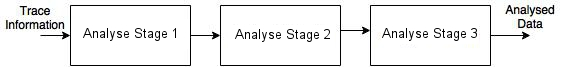
\includegraphics[width=\textwidth]{Pipeline.jpg}
\caption{\DIFaddFL{Trace information goes in at the start of the pipeline. After each stage there should be a reduction of comparisons that the next stage has to complete. The last stage should be the most computationally heavy.}}
\label{fig:pipeline}
\end{figure}
\DIFaddend 

\DIFdelbegin %DIFDELCMD < \begin{tabular}{|l|l|l|}
%DIFDELCMD < \hline
%DIFDELCMD < {\bf %%%
\DIFdel{Previous State}%DIFDELCMD < } & {\bf %%%
\DIFdel{Current State}%DIFDELCMD < } & {\bf %%%
\DIFdel{Operation}%DIFDELCMD < }                      \\ \hline
%DIFDELCMD < %%%
\DIFdel{-                    }%DIFDELCMD < & %%%
\DIFdel{kitten              }%DIFDELCMD < & %%%
\DIFdel{-                                    }%DIFDELCMD < \\ \hline
%DIFDELCMD < %%%
\DIFdel{kitten               }%DIFDELCMD < & %%%
\DIFdel{kitcen              }%DIFDELCMD < & %%%
\DIFdel{Substitution of `t'with `c'         }%DIFDELCMD < \\ \hline
%DIFDELCMD < %%%
\DIFdel{kitcen               }%DIFDELCMD < & %%%
\DIFdel{kitchen             }%DIFDELCMD < & %%%
\DIFdel{Insertion of `h' between `c' and `e'}%DIFDELCMD < \\ \hline
%DIFDELCMD < \end{tabular}
%DIFDELCMD < %%%
%DIFDELCMD < \caption{%
{%DIFAUXCMD
\DIFdel{Using levenshtein edit distance algorithm to transform kitten to kitchen.}}
%DIFAUXCMD
%DIFDELCMD < \label{levenTable}
%DIFDELCMD < \end{table}
%DIFDELCMD < %%%
\DIFdelend \DIFaddbegin \subsection{\DIFadd{Saving to the Network}}
\DIFadd{To execute the analysis on a grid computing system, the test data had to accessible on the School of Engineering's local network. To achieve this, the data retrieved by the tool was saved to the local network. Not only did it allow for the analysis to be executed on the grid system, it also it allowed for the data to be reanalysed without having to re execute the test suite. 
}\DIFaddend 

\DIFaddbegin \section{\DIFadd{Tracing Parameter Values}}
\label{parameterTrace}
\DIFadd{The related work in the research area has explored using statement coverage while ignoring the parameter values of each method. It could be argued that due to knowing the statement path, parameters are irrelevant as you know the path the method will take, and parameters do not add any more information. When tracing at method level rather than at the statement, these become crucial to determine the degree of redundancy between test cases. Parameters give insight into the execution paths that will be taken and act as a proxy to the statement information without storing the same amount of the data.
}

\DIFadd{There were two variations of parameters that were considered to trace. Firstly, primitive types only. By running test experiments on the benchmarks, the use of primitives showed that only a limited number of parameters were collected. The parameters collected had a limited effect on the number of false positives identified and time taken. The second approach is to use reflection. Reflection is the ability to examine and modify objects at run time \mbox{%DIFAUXCMD
\cite{oraclereflection}
}%DIFAUXCMD
. Since AspectJ gives direct access to the object's in the parameters, reflection can be used. By using reflection, the fields of the objects are retrieved and returned in a string to represent the state of the object. This string is then examined to remove any Java object reference location and stored.
}

\DIFadd{The most common use case of the tool is expected to use parameters therefore it was decided to optimize this through storing the data with parameters. The optimization involved saving the parameters with the trace information. If parameters value is set to false, the parameters have to be split off rather than added on. This means that setting the parameters to false would increase the set up time.
}

\DIFaddend \section{Weighting}
Maurer et al. \cite{koochakzadeh2009test} and Robinson et al. \cite{li2008static} found that test \DIFdelbegin \DIFdel{cases }\DIFdelend \DIFaddbegin \DIFadd{suites }\DIFaddend often had a set of methods that were in every test, such as setup and tear down. These common methods could create false positives. To understand why, a redundant test is one where it is nearly or exactly a replication of another test. Since each method call within a spectra has the same weighting, the more setup and teardown calls made means that the execution stage has decreased weighting overall. \DIFaddbegin \DIFadd{We can see an example of this in Figure \ref{fig:weightingdiagram}. The figure shows test cases with different proportions of setup and tear down in relation in the execution stage. The figure also shows how the size of the test case may effect the proportion.
}

\DIFaddend Two different variations of weighting were considered. The first variation involved \DIFdelbegin \DIFdel{having }\DIFdelend \DIFaddbegin \DIFadd{giving }\DIFaddend each method execution \DIFdelbegin \DIFdel{be given }\DIFdelend a weighting based on \DIFdelbegin \DIFdel{it's }\DIFdelend \DIFaddbegin \DIFadd{its }\DIFaddend call frequency, the higher the frequency, the lower the weighting. This would cause the more common methods to have less impact on the final result, but not be removed completely. The other variation that was considered, and used, was completely removing the most used method calls for each test case. This involved removing every method execution that was more than 80 percent of the most frequent method call. \DIFdelbegin \DIFdel{The }\DIFdelend \DIFaddbegin \DIFadd{During initial experiments, the }\DIFaddend first variation was found to have less impact\DIFdelbegin \DIFdel{, with some of the method calls having a substantially larger number of method calls compared to the less frequent, it was difficult to find a weighting system that worked well for every test case, often the more }\DIFdelend \DIFaddbegin \DIFadd{. The reason was that the }\DIFaddend frequent method calls were still having a large impact, even with a lower weighting. \DIFaddbegin \DIFadd{This meant that each benchmark needed different weightings therefore it was difficult to find a solution that could be applied on every benchmark.
}\DIFaddend 

Another decision was the scope of the weighting, either it was calculated per test case or \DIFdelbegin \DIFdel{globally}\DIFdelend \DIFaddbegin \DIFadd{test suite}\DIFaddend . The issue with \DIFdelbegin \DIFdel{using global }\DIFdelend \DIFaddbegin \DIFadd{calculating per suite }\DIFaddend was that if the benchmark contained a mixture of large and small tests, \DIFdelbegin \DIFdel{then the use of global }\DIFdelend \DIFaddbegin \DIFadd{this }\DIFaddend could cause the smaller benchmarks to be reduced to a minimal number of method calls. \DIFaddbegin \DIFadd{The minimal number of method calls was often not enough information to present the test in a representable state. }\DIFaddend A per test case weighting was desired to reduce the issue of test cases being reduced to a minimal size.
\DIFaddbegin 

\begin{figure}[h]
\includegraphics[width=14cm, height=6cm]{weightingdiagram.png}
\caption{\DIFaddFL{A diagram showing how the different size of the test case can be affected by setup and teardown methods.}}
\label{fig:weightingdiagram}
\end{figure} \DIFaddend \newpage 
 \newpage \chapter{Results and Discussion}\label{C:results}\label{C:evaluation}

The following section reports on the outcome of several experiments that explore the use of our framework \DIFdelbegin \DIFdel{through }\DIFdelend \DIFaddbegin \DIFadd{on }\DIFaddend a realistic benchmark suite. The key factors of interest are -- the time taken, number of comparisons, the types of redundant tests identified and the overall cost of performance (time) vs precision (tests identified \& types identified). \todo{Link back to req?}

There are two points that the reader needs to be aware of. Firstly, in the significant tables below, a `+' represents that significant increase, `-' significant decrease and `=' represents no significant difference. Secondly, the graphs are displayed using a logarithm scale.

\section{Method}

The experiment method is key to producing believable and reproducible results. Before the experiment could be conducted, the data for each benchmark had to be retrieved. This involved setting the benchmark up locally and then executing the tests with the AspectJ class loader. The data was then run on a grid computing system. After the results had been returned, a Wilcoxon signed rank test \cite{wilcoxon1945individual} was used to determine whether the results were significantly different or not. The significant level used was 95\% with a null hypothesis of the two samples median being equal. Overall, \DIFdelbegin \DIFdel{a total of seven different property }\DIFdelend \DIFaddbegin \DIFadd{seven different }\DIFaddend settings were run per benchmark with each \DIFdelbegin \DIFdel{property }\DIFdelend setting being run 30 times.

The goals of this paper as mentioned in Section \ref{C:intro} are the creation of a framework to identify redundant test cases and experimenting \DIFdelbegin \DIFdel{the }\DIFdelend \DIFaddbegin \DIFadd{with }\DIFaddend different techniques on realistic benchmarks. The rest of this \DIFdelbegin \DIFdel{section }\DIFdelend \DIFaddbegin \DIFadd{chapter }\DIFaddend explores the experiments conducted to give guidance to the users of the \DIFdelbegin \DIFdel{framework}\DIFdelend \DIFaddbegin \DIFadd{tool}\DIFaddend .

\section{Environmental Methodologies}
\label{enviro}
As previously discussed in Section \ref{performanceEvalBG} there are a variety of challenges that present themselves when using Java to evaluate performance. These challenges are discussed throughout the following section.

\subsection{Grid Computing}
A grid computing system was used to execute the data analysis, with a total of 150 jobs queued on the grid at a single time. When using a grid system it is important to ensure that all the machines used are the same for every experiment. The grid allowed for particular types of machines to be specified -- 8gb \DIFdelbegin \DIFdel{total }\DIFdelend \DIFaddbegin \DIFadd{ddr3 }\DIFaddend ram, Linux 4.0.5 64 bit system and an \DIFdelbegin \DIFdel{i5}\DIFdelend \DIFaddbegin \DIFadd{Intel Core i7-3770 CPU running @ 3.40GHz}\DIFaddend .

\subsection{Measuring Time}
The time taken is an important variable in evaluating the performance of a tool. In Java, this can be achieved by accessing a system method that returns the total time in milliseconds from 1970 00:00:00 UTC to the current time. Taking this time before the analysis, and subtracting from the time after the analysis gives the total time taken. This notation of time is defined as wall clock time. Utilising a grid system presents difficulties with using the wall clock time to measure the time taken. 

As mentioned in Section \ref{C:related}, when a job is run on the grid system, there is potential for the machine to be paused. If wall time were to be used, the time that the process is paused would also be included. To resolve this issue, the notation of CPU time was used. The CPU time is the measure of time in nanoseconds that the computer program spent on the CPU. Another \DIFdelbegin \DIFdel{issue in regard to time taken }\DIFdelend \DIFaddbegin \DIFadd{concern is }\DIFaddend if a user logs in during analysis, \DIFdelbegin \DIFdel{is the programs }\DIFdelend \DIFaddbegin \DIFadd{the tool's }\DIFaddend RAM could potentially be moved into virtual memory. This is dependent on the amount of RAM that the user needs. \DIFaddbegin \DIFadd{When the user logs out, the tool will restart and any information lost will need to be recalculated by the tool. }\DIFaddend Both these issues were limited by running the tests overnight when users were unlikely to log \DIFaddbegin \DIFadd{in}\DIFaddend .

When measuring the time taken to analyse, the start up cost was not taken into account. Running up to 150 jobs meant that a large number of applications would be attempting to access a single data file at a single time. This stress on the system introduces a large amount of non-deterministic behaviour. Removing the start up cost avoided this issue.

\subsubsection{Heap Size}
The heap is the location that the JVM uses to store objects that are produced during the execution of an application. The amount of heap that was allocated to the JVM was 6gb \DIFdelbegin \DIFdel{for every benchmark over }\DIFdelend \DIFaddbegin \DIFadd{on every benchmark for }\DIFaddend every run.

\subsection{Software Environment}

A concurrent-mark-sweep garbage collection strategy (default) was used. This approach uses multiple threads to scan the heap, mark unused objects and recycle them \cite{oracle2015}. It allows for a high throughput however, tends to use more CPU time than other strategies. This was deemed worth the trade off as memory was the bottleneck rather than \DIFdelbegin \DIFdel{CPU and increasing the throughput was more important}\DIFdelend \DIFaddbegin \DIFadd{the CPU}\DIFaddend .

\section{Benchmarks}
\label{S:bench}
The benchmarks had to be realistic real world projects. They were located by looking at popular Java frameworks, Github repositories and David Pearce's personal projects. For a benchmark to be considered, it had to be Java based, have a reasonable number of tests (40+) and \DIFdelbegin \DIFdel{was open source}\DIFdelend \DIFaddbegin \DIFadd{open sourced}\DIFaddend , while Ant and Gradle built projects were favoured due to their easier build process.

A variety of test types and sizes of benchmarks were examined. A range of sizes were used in order to fully evaluate the framework. The two ranges of benchmark sizes can be found in Table \ref{large_test} and Table \ref{small_test}, large and small respectively. Although \DIFdelbegin \DIFdel{method execution details approach }\DIFdelend \DIFaddbegin \DIFadd{the type of data retrieved }\DIFaddend is aimed toward larger test suites, it would be expected that \DIFaddbegin \DIFadd{the }\DIFaddend size will have no \DIFdelbegin \DIFdel{correlation to the metrics examined}\DIFdelend \DIFaddbegin \DIFadd{effect on the outcome of the experiments}\DIFaddend . A range of test types were also chosen, David J Pearce's projects contain end to end tests which run through a whole module at once, while the rest attempt to test units of code at a time. Having a range of test types gives a wider evaluation view and gives insight into potential situations where different settings may not be helpful in achieving the aim.

The larger benchmarks that produced up to 100,000 method calls per test required a large amount of memory to store the details during data retrieval. Without the use of a database, this limited the number of test cases that could be collected. Whiley and Ant were the benchmarks that did not have all there tests executed.  

\begin{table}[]
\centering

\begin{tabular}{|l|l|l|l|}
\hline
{\bf Benchmark}       &  {\bf Number of Tests} & {\bf Type of tests} & {\bf Authors}   \\ \hline
Whiley - Wyc         &       &    End to End      & David J Pearce          \\ \hline
Spring - Core   &       &    Unit Tests      & Community \\ \hline
Metric-x - Core &       &    Unit Tests      & Community \\ \hline
Jasm              &             &    End to End      & David J Pearce \\ \hline

\end{tabular}
\caption{Large Test Suites}
\label{large_test}
\end{table}

\begin{table}[]
\centering
\begin{tabular}{|l|l|l|l|}
\hline
{\bf Benchmark}   & {\bf Number of Tests} & {\bf Type of tests} & {\bf Authors}  \\ \hline
Ant             &       &    Unit Tests      & Community \\ \hline
Imcache &           &    End to End        & Community \\ \hline
\end{tabular}
\label{small_test}
\caption{Small Test Suites}
\end{table}

\section{Experiment \rom{1} - Pipeline Length Comparison}
\label{sec:pipelineEva}

\subsection{Motivation}
The pipeline size has impact on each factor of interest. Selecting a pipeline too small or too large will have varying negative effects on these. This experiment explores this trade off and the number of pipelines that should be used with the benchmarks.

\begin{hyp}
Increasing the number of pipeline's improves the factors of interest
\end{hyp}

\begin{hyp}
Increasing the number of pipeline's leads to no difference between the output redundant test cases
\end{hyp}

\subsection{Settings}
There were two different pipeline size's tested, two and three respectively. For both size's, the final pipeline stage was the same. It is noted that a single pipeline comparison was left out due to the amount of memory and time taken to finish analysing.

\begin{itemize}
\item Difference between runs: Pipeline size
\end{itemize}

\subsection{Results}

The significant table for comparing the use of pipeline of size two \DIFdelbegin \DIFdel{vs }\DIFdelend \DIFaddbegin \DIFadd{and }\DIFaddend size three is shown in Table \ref{pipelinesig}. It shows that there was a mixture of results for the total time taken to analyse the data. Metrics-x, Ant, Spring and Jasm performed significantly better with a pipeline of size three in comparison to size two. Imcache had no significant difference and Whiley performed significantly worse with a pipeline of size three in comparison to size two. Every benchmark \DIFdelbegin \DIFdel{has }\DIFdelend \DIFaddbegin \DIFadd{had }\DIFaddend no significant difference between the number of redundant tests identified, every benchmark produced the exact same number of redundant tests in both pipeline size of two and three.

A chart showing how each benchmark reacted to the change in the pipeline size is shown in Figure \ref{fig:pipelinegraph}. It shows the number of test case comparisons that the final stage of the pipeline \DIFdelbegin \DIFdel{has }\DIFdelend \DIFaddbegin \DIFadd{had }\DIFaddend to conduct.

\begin{table}[h]
\centering
\begin{tabular}{|l|l|l|}
\hline
{\bf }          & {\bf Total Time} & {\bf Redundant Tests Identified} \\ \hline
{\bf Whiley}    & +                & =                           \\ \hline
{\bf Jasm}      & -                & =                           \\ \hline
{\bf Ant}       & -                & =                           \\ \hline
{\bf Spring}    & -                & =                           \\ \hline
{\bf Imcache}   & =                & =                           \\ \hline
{\bf Metrics-x} & -                & =                           \\ \hline
\end{tabular}
\caption{A table showing the significant relationship between the use of pipeline of size two with pipeline of size three for each benchmark}
\label{pipelinesig}
\end{table}

\begin{figure}[h]
\begin{center}
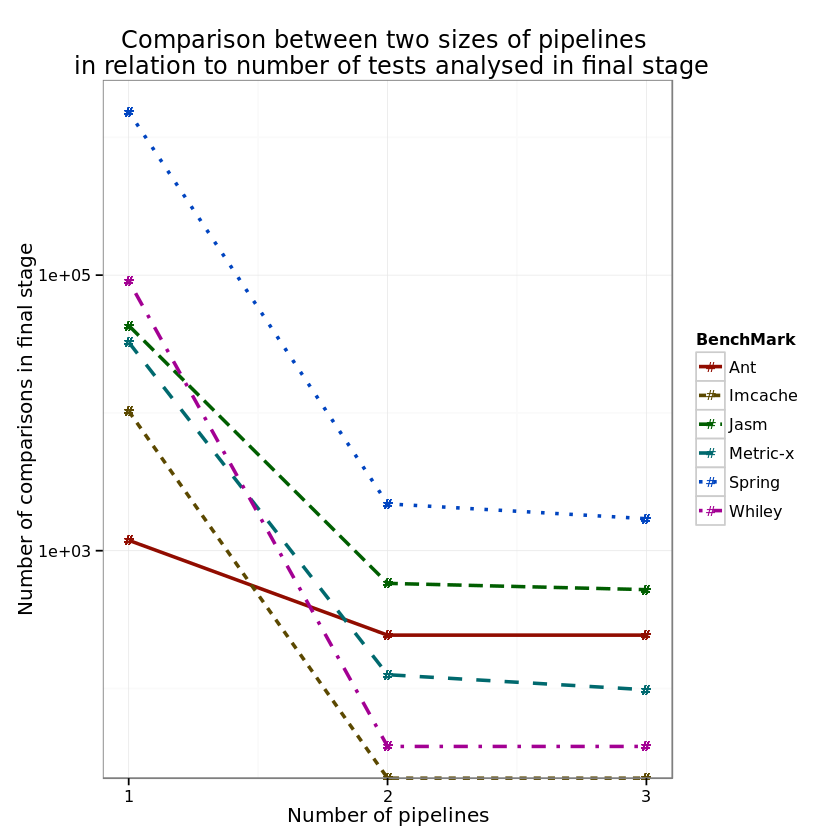
\includegraphics[height=10cm, width = 14.5cm]{Pipeline.png}
\end{center}
\caption{A figure showing the effect that using pipelines has on the number of comparisons that the final stage (Most computationally heavy) has to do.}
\label{fig:pipelinegraph}
\end{figure}

\subsection{Discussion}

The first hypothesis states an increase in the pipeline size will improve the factors of interest. \DIFdelbegin \DIFdel{An }\DIFdelend \DIFaddbegin \DIFadd{The purpose of an }\DIFaddend increase in the pipeline size \DIFdelbegin \DIFdel{aimed }\DIFdelend \DIFaddbegin \DIFadd{was }\DIFaddend to reduce the number of comparisons that the next stage had to perform. This \DIFdelbegin \DIFdel{in turn decreased }\DIFdelend \DIFaddbegin \DIFadd{reduction decreased the }\DIFaddend memory and time taken. \DIFdelbegin \DIFdel{Immediately }\DIFdelend \DIFaddbegin \DIFadd{Inspecting Figure \ref{fig:pipelinegraph}, }\DIFaddend it becomes clear that that pipeline size does improve the factors, but \DIFdelbegin \DIFdel{doesn't }\DIFdelend \DIFaddbegin \DIFadd{does not }\DIFaddend scale in every benchmark. \DIFdelbegin \DIFdel{This becomes visible when examining Figure \ref{fig:pipelinegraph}. }\DIFdelend Every two or three stage pipeline is a significant improvement on a single stage, however the majority of \DIFaddbegin \DIFadd{the }\DIFaddend benchmark's perform better \DIFdelbegin \DIFdel{for }\DIFdelend \DIFaddbegin \DIFadd{with }\DIFaddend a two stage over a three. These results imply that the benchmarks that took less time using a two stage, were spending more time on the second stage than they were saving from the reduced number of comparisons in the third stage. 

Two situations which would cause more time to be spent on the second stage than was saved in the third stage are proposed. Firstly, each benchmark had it's own level of redundancy that was being looked for, this was dependent on how each benchmark reacted to different levels. Benchmarks with unit tests needed to have a higher level in comparison to benchmarks with end to end. Since each \DIFdelbegin \DIFdel{benchmark }\DIFdelend had their own percentage, this implies \DIFdelbegin \DIFdel{that each benchmark also has its }\DIFdelend \DIFaddbegin \DIFadd{they also have their own }\DIFaddend optimal settings for the second pipeline. The settings were chosen by experimenting with different options, therefore a inefficient second pipeline would have contributed to \DIFdelbegin \DIFdel{it}\DIFdelend \DIFaddbegin \DIFadd{the result}\DIFaddend .

The second reason is that there may be little difference between the \DIFdelbegin \DIFdel{second pipeline and third pipeline}\DIFdelend \DIFaddbegin \DIFadd{outcome from the second and third pipelines}\DIFaddend . An example is shown in \DIFdelbegin \DIFdel{Appendix }\DIFdelend \DIFaddbegin \DIFadd{Figure }\DIFaddend \ref{fig:pipelinecomp}. Examining the three stage pipeline, it shows the first pipeline causes a large reduction in the number of comparisons needed implying that the tests are highly separable. Inserting the second stage, a limited amount of reduction occurs while being computationally heavy and passes the majority of test cases into the third and most computationally heavy stage. \todo{Talk about cost here.} This \DIFdelbegin \DIFdel{leads to }\DIFdelend \DIFaddbegin \DIFadd{creates }\DIFaddend a situation where the number of identified redundant test cases has little change from stage two to three. This leads me to accept the first hypothesis, that increasing the pipeline size improves the factors of interest, however the optimal length is different for each benchmark.

The second hypothesis is that there is no difference between the number of output test cases. As expected, each benchmark had no significant change. If there were a change between the two pipelines with the same final stage settings could imply two things. Firstly, there is a bug in the code. Secondly, the second pipeline stage is more specific than the \DIFdelbegin \DIFdel{last}\DIFdelend \DIFaddbegin \DIFadd{third}\DIFaddend . Since both \DIFdelbegin \DIFdel{the second stage and third stage }\DIFdelend \DIFaddbegin \DIFadd{pipelines of size two and three }\DIFaddend share the same \DIFaddbegin \DIFadd{settings in }\DIFaddend final stage, \DIFdelbegin \DIFdel{this would cause the last stage to be redundant and the redundant tests different to that of the two stage pipeline}\DIFdelend \DIFaddbegin \DIFadd{for the pipeline of size three, the second stage is a higher percentage than the final, this would cause a different output between the two sizes}\DIFaddend . 

\DIFaddbegin \begin{figure}[h]
\centering
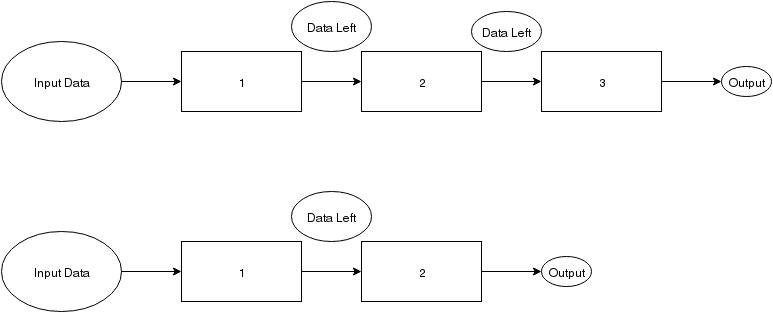
\includegraphics[width=\textwidth,height=8cm]{PipelineComp.png}
\caption{\DIFaddFL{The circle size represents the data that is left in the pipeline. The figure shows that the difference that is between a two stage pipeline and a three stage only has limited room for a reduction in test cases identified. This shows that the time taken to run the extra pipeline costs more than it saves.}}
\label{fig:pipelinecomp}
\end{figure}

\DIFaddend \section{Experiment \rom{2} - K Depth Comparison}
\label{kdepthcomp}
\subsection{Motivation}
One of the abilities of the framework is to trace the K depth specified. This experiment is to determine the impact that altering the depth of K has on the overall cost. 

\begin{hyp}
\DIFdelbegin \DIFdel{Increasing the K Depth improves the precision is worth the trade off in }\DIFdelend \DIFaddbegin \DIFadd{The precision improvement from increasing K Depth outweighs the }\DIFaddend performance decrease.
\end{hyp}

\subsection{Settings}
There are three K depth's explored, one, two and three respectively.

\begin{itemize}
\item Difference between runs: K Depth
\end{itemize}

\subsection{Results}
Ant, Whiley and Spring appear to be the most responsive to the depth of K as shown in Figure \ref{fig:kdepthgraph} while the rest have limited change. Appendix \ref{fig:kdepthtime} shows the differences in time taken. Overall, for every benchmark there wasn't a large amount of change between them however it shows that as the K depth increases, the time taken increases.

\begin{figure}[h]
\begin{center}
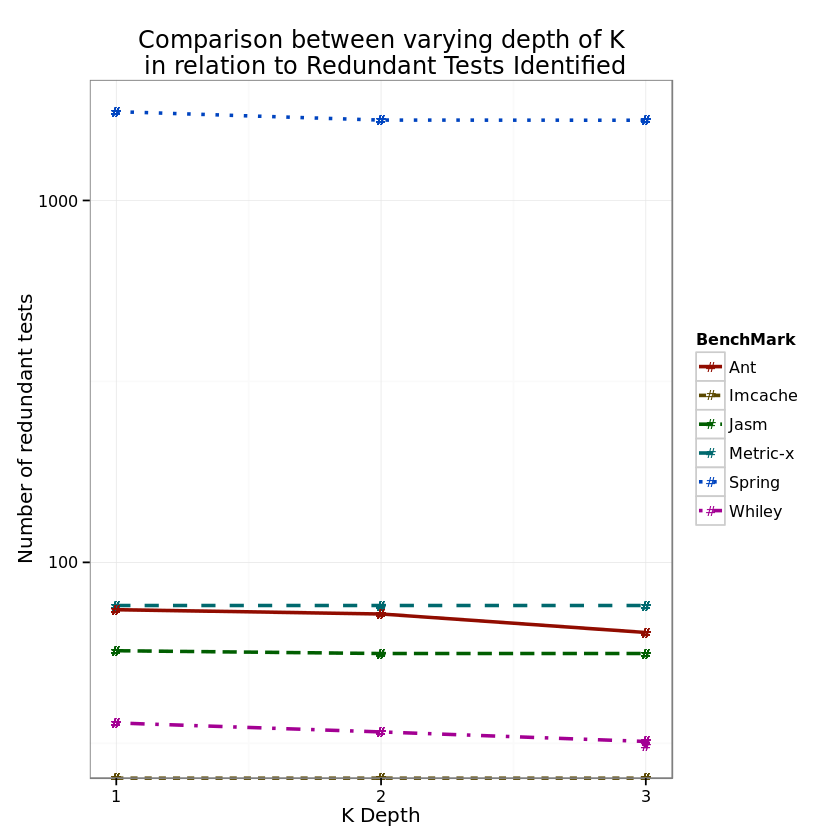
\includegraphics[height=10cm, width = 14.5cm]{KDepth.png}
\end{center}
\caption{A figure showing the effect that a change in the depth of the calling context has on the number of redundant tests are identified.}
\label{fig:kdepthgraph}
\end{figure}

\subsection{Discussion}
Increasing the depth of the calling context increases the amount of data that is analysed, intuitively making it more difficult for test cases to be the same. This should be reflected through a reduction in the overall tests identified. The extra data used is going cause extra analysis, this implies an increase in the time taken as calling context depth increases. It is expected that the precision increase is worth the performance decrease.

Examining Figure \ref{fig:kdepthgraph}, it shows that the number of redundant tests is only slightly decreased as the K depth increases. This \DIFdelbegin \DIFdel{may show }\DIFdelend \DIFaddbegin \DIFadd{shows }\DIFaddend several things. Firstly, it \DIFdelbegin \DIFdel{may imply }\DIFdelend \DIFaddbegin \DIFadd{implies }\DIFaddend that when no other settings such as weighting or parameters are used, then the depth has limited effect on the redundant test cases identified. Secondly, the number of comparisons that were output from the first pipeline stage may cause there to be a limited differentiation. When the first pipeline stage outputs a low number of comparisons, then the final number of redundant tests identified would be similar regardless of the K depth specified, similar to the situation in Section \ref{sec:pipelineEva}. This occurs in Whiley\DIFdelbegin \DIFdel{and }\DIFdelend \DIFaddbegin \DIFadd{, }\DIFaddend Metric-x\DIFaddbegin \DIFadd{, Imcache and Jasm}\DIFaddend . 

Increasing the depth of K has varying effect's on the time taken to analyse a benchmark. The differences are shown in Appendix \ref{fig:kdepthtime}. It shows that Ant, Imcache and Whiley have larger differences than the rest, however in the perspective of time these equate to around half a minute difference. Although increasing the depth has an smaller effect than expected on precision, the impact on time taken isn't substantial. Taking this into account, I can accept the hypothesis with the results implying that for some projects the calling context does not have to be particularly deep.

\section{Experiment \rom{3} - Parameter Comparison}
\label{sec:param}

\subsection{Motivation}
Parameters show the different contexts that a method was being called in. Retrieving this information gives us more confidence in determining whether two tests are redundant. \DIFdelbegin \DIFdel{This shows the importance of parameters and the }\DIFdelend \DIFaddbegin \DIFadd{The }\DIFaddend experiment explores the \DIFdelbegin \DIFdel{increase in }\DIFdelend \DIFaddbegin \DIFadd{impact on }\DIFaddend performance and precision.

\begin{hyp}
Utilising parameters \DIFdelbegin \DIFdel{increase }\DIFdelend \DIFaddbegin \DIFadd{increases }\DIFaddend the time taken \DIFdelbegin \DIFdel{of the framework }\DIFdelend in comparison to a \DIFdelbegin \DIFdel{standard }\DIFdelend three stage pipeline\DIFaddbegin \DIFadd{.
}\DIFaddend \end{hyp}

\begin{hyp}
Utilising parameters \DIFdelbegin \DIFdel{increase the precision of the framework }\DIFdelend \DIFaddbegin \DIFadd{increases the precision }\DIFaddend in comparison to a \DIFdelbegin \DIFdel{standard }\DIFdelend three stage pipeline\DIFaddbegin \DIFadd{.
}\DIFaddend \end{hyp}

\subsection{Settings}
The use of parameters is compared directly to the pipeline size three settings.

\begin{itemize}
\item Difference between runs: Parameters used during analysis
\end{itemize}

\subsection{Results}
The significant table for comparing parameters and no parameters is shown in Table \ref{parametersig}. It shows that there was a negative relation (increase) for every benchmark in regard to time taken. Every benchmark had a significantly positive effect (decrease) on the number of redundant test cases identified. This is not the case in Imcache due to it having zero redundant test cases identified in both, therefore no difference between the two.

\begin{table}[h]
\centering
\begin{tabular}{|l|l|l|}
\hline
{\bf }          & {\bf Total Time} & {\bf Redundant Tests Identified} \\ \hline
{\bf Whiley}    & +                & -                           \\ \hline
{\bf Jasm}      & +               & -                          \\ \hline
{\bf Ant}       & +                & -                           \\ \hline
{\bf Spring}    & +                & -                           \\ \hline
{\bf Imcache}   & +                & =                           \\ \hline
{\bf Metrics-x} & +                & -                           \\ \hline
\end{tabular}
\caption{A table showing the significant relationship between the use of parameters and no parameters for each benchmark}
\label{parametersig}
\end{table}

\begin{figure}[H]
\begin{center}
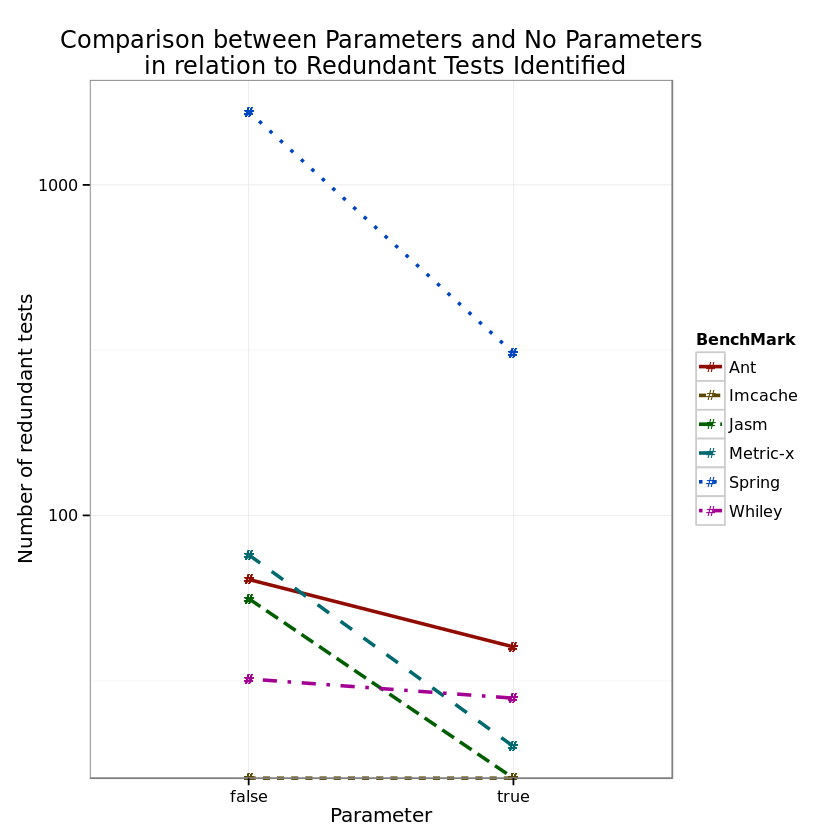
\includegraphics[height=10cm, width = 14.5cm]{Parameters.png}
\end{center}
\caption{A figure showing the effect that using parameters has on the number of redundant tests are identified.}
\label{fig:paramgraph}
\end{figure}

\subsection{Discussion}
Two factors have to be taken into account when discussing the impact of parameters on the time taken. Firstly, it is intuitive that analysing the extra data generated increases the time. The amount of increase is interesting, parameters only add extra computation when the method execution of the given K is exactly the same. For example, if test execution is $A ->  B ->  C$ is compared to $A ->  B ->  F$. Then the parameter won't be taken into account and therefore have limited effect on the time taken. 

The amount of time that the VM spends garbage collecting would also increase the time taken, due to increased amount of information in memory, the garbage collection process will have to execute more frequently for the analysis to continue to run. This would cause non-deterministic attributes to be increased. Examining Appendix \ref{fig:paramtime} -- Ant, Imcache, Jasm and Spring appear to affected by this due to the increased variance. This creates the hypothesises that parameters \DIFdelbegin \DIFdel{decrease }\DIFdelend \DIFaddbegin \DIFadd{increase }\DIFaddend the precision and \DIFdelbegin \DIFdel{increase }\DIFdelend the total time taken. 

The significant Table \ref{fig:paramgraph} matches what is expected. For every benchmark, using parameters significantly increases the time taken. Examining Appendix \ref{fig:paramtime} shows how the benchmarks react with more detail. The most interesting would be \DIFdelbegin \DIFdel{JASM}\DIFdelend \DIFaddbegin \DIFadd{Jasm}\DIFaddend . Without parameters, it analyses the data in less than one minute, with parameters, it takes just under five minutes. This may be indicative of the results discussed in Section \ref{kdepthcomp}. With K depth having little effect on a reduction in comparisons, the number of tests that match the K depth of three is higher than expected. This effect led to parameter information being examined more often, sequentially causing an increase in time taken. \todo{A factor that may have an accumulate effect} is related to the setup methods. If the set up methods are a large majority of the method calls, and match each other for the K depth, this would further increase the time taken. This allows us to accept hypothesis 4.

Every benchmark caused a significant decrease in the number of redundant test cases. Looking at Figure \ref{fig:paramgraph}\DIFdelbegin \DIFdel{shows }\DIFdelend \DIFaddbegin \DIFadd{, it confirms }\DIFaddend that every benchmark reacted with a substantial decrease in redundant tests identified, with Whiley being the least affected. This reiterates the discussion in Section \ref{kdepthcomp} that K depth is not enough of a factor to identify redundant test cases. It is expected that \DIFdelbegin \DIFdel{identified tests decreases}\DIFdelend \DIFaddbegin \DIFadd{the number of false positives decrease}\DIFaddend , inspecting Table \ref{whileycoding} and \ref{metriccoding} gives insight into the types of tests identified. The Whiley benchmark coding shows that parameters remove the limited redundant tests as well as different array values. The Metric-x coding \DIFdelbegin \DIFdel{shows the influence that parameters has. Parameters reduce the }\DIFdelend \DIFaddbegin \DIFadd{demonstrate a reduction in the }\DIFaddend number of the different parameter value tests identified substantially, from 52 to 8. \DIFdelbegin \DIFdel{These coding }\DIFdelend \DIFaddbegin \DIFadd{Taking these coding tables into account, }\DIFaddend allow us to accept hypothesis 3.

\section{Experiment \rom{4} - Weighting Comparison}
\label{sec:weight}

\subsection{Motivation}
Utilising weighting is an attempt to remove any false positive tests identified. The experiment attempts to identify if weighting has any potential to remove these false positives, while exploring the impact on performance.

\begin{hyp}
Weighting decreases the number of false positives compared to a standard three stage pipeline
\end{hyp}

\begin{hyp}
Weighting decreases the time taken compared to a standard three stage pipeline
\end{hyp}

\subsection{Settings}
The use of weighting is compared directly to the pipeline size three settings.

\begin{itemize}
\item Difference between runs: Weighting Used
\end{itemize}

\subsection{Results}
The significant table for comparing the use of weighting is shown in Table \ref{weightingsig}. There are a mixture of results in regard to the total time taken -- Whiley, Ant and Imcache had a significantly negative relation and weighting increased the time taken to analyse. Jasm, Spring and Metric-x had a significantly positive relation and weighting decreased the time taken to analyse. The majority -- Whiley, Ant, Jasm and Metrics-x had a significantly positive relation in regard to the number of redundant tests identified, showing a decrease in the number identified when weighting was applied. Spring was the only benchmark where weighting had a significantly negative impact.

\begin{table}[h]
\centering


\begin{tabular}{|l|l|l|}
\hline
{\bf }          & {\bf Total Time} & {\bf Redundant Tests Identified} \\ \hline
{\bf Whiley}    & +                & -                           \\ \hline
{\bf Jasm}      & -                & -                           \\ \hline
{\bf Ant}       & +                & -                           \\ \hline
{\bf Spring}    & -                & +                           \\ \hline
{\bf Imcache}   & +                & =                           \\ \hline
{\bf Metrics-x} & -                & -                           \\ \hline
\end{tabular}
\caption{A table showing the significant relationship between the use of weighting and no weighting for each benchmark}
\label{weightingsig}
\end{table}


\begin{figure}[h]
\begin{center}
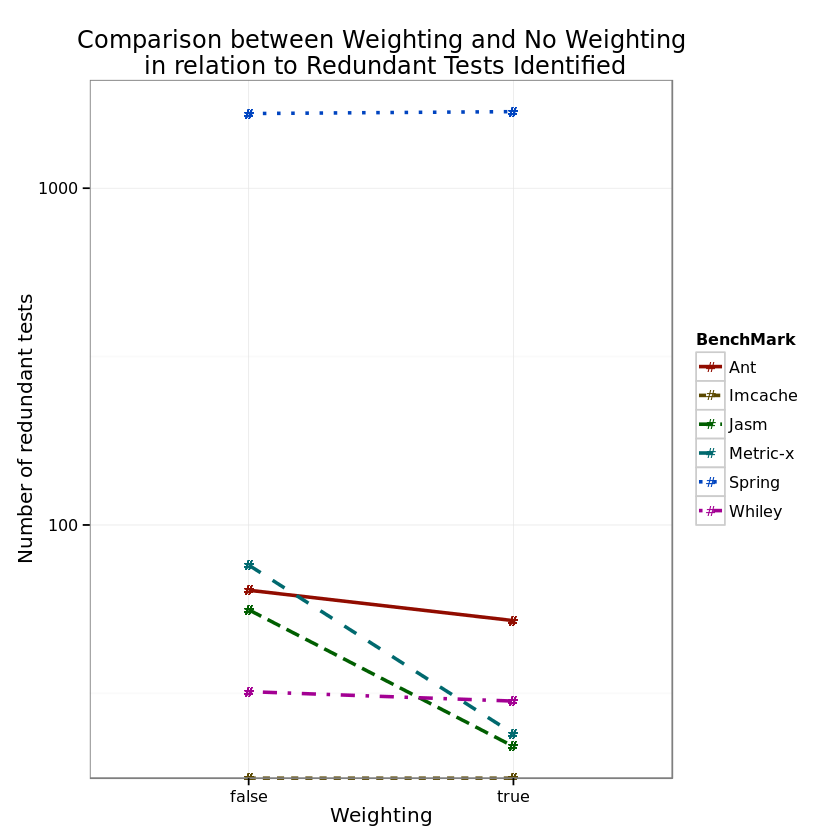
\includegraphics[height=10cm, width = 14.5cm]{Weighting.png}
\end{center}
\caption{A figure showing the effect that using weighting has on the number of redundant tests are identified.}
\label{fig:weightgraph}
\end{figure}

\subsection{Discussion}
As previously discussed in Section \ref{C:related}, much of the related work encountered difficulties with test cases sharing setup and teardown method calls, resulting in a high false positive rate. Intuitively this makes sense when the test cases are small in comparison to the setup and teardown methods where the setup and teardown methods \DIFdelbegin \DIFdel{are a larger }\DIFdelend \DIFaddbegin \DIFadd{represent a large }\DIFaddend majority of the \DIFdelbegin \DIFdel{tests }\DIFdelend \DIFaddbegin \DIFadd{test }\DIFaddend data. The approach of removing a portion of the most executed method calls meant that the amount of data that would be compared decreases. This should reflect onto the results by showing a decrease in the time taken, as per hypothesis 7. The effect that it has on the number of redundant test cases should be dependent on the benchmark when weighting is used. This is because removing the most common tests should imply an decreased false-positive rate, but also may increase the number of actual redundant tests picked up. \DIFdelbegin \DIFdel{To examine }\DIFdelend \DIFaddbegin \DIFadd{The precision is of interest when examining }\DIFaddend the cause effect of weighting, \DIFdelbegin \DIFdel{the precision to validate or invalidate }\DIFdelend \DIFaddbegin \DIFadd{this is reflected by }\DIFaddend hypothesis 6.

Table \ref{weightingsig} shows a mixture of results in regard to the total time taken. Two out of the three benchmarks that had a significant increase in the total time were small benchmarks. This may imply that the size of the benchmark has some relation to the effect of weighting on the time taken. One reason \DIFdelbegin \DIFdel{may be }\DIFdelend \DIFaddbegin \DIFadd{is }\DIFaddend that weighting is calculated once per test case per analysis stage. The weighting calculation has a linear relation with the number of test cases. In comparison, every test case is compared to every other, therefore a factorial relation with the number of test cases. Since the factorial relation is closer to linear, the smaller the number of redundant test cases. Then the smaller the number, the more impact the linear weight calculation has on the overall time taken. This may explain a relation between size and time taken. Examining the overall impact from weighting on the time taken in Appendix \ref{fig:weighttime} allows us to invalidate hypothesis 7 as there is no general consensus between benchmarks.

A reduction in the false positive rate was weightings primary goal. Spring was the only benchmark that significantly increased the number of redundant test cases identified. The other benchmarks had a significant decrease. At first, this makes it appear that by using weighting it may solve some of the issues that were identified in \cite{koochakzadeh2009test} \cite{li2008static}. To confirm this, examining Table \ref{whileycoding} and \ref{metriccoding} will give insight into the effect of weighting. Comparing the two columns for the Whiley coding, Pipeline 2 and Weighting, the only difference is the removal of the two limited redundancy test cases that were picked up by Pipeline 2. The weighting is able to remove the test cases that have similar set up and tear down methods, but fails to reduce the number of other redundancies. By removing the method executions that were common throughout the benchmarks, this \DIFdelbegin \DIFdel{lead }\DIFdelend \DIFaddbegin \DIFadd{led }\DIFaddend to a decrease in \DIFdelbegin \DIFdel{false-positive }\DIFdelend \DIFaddbegin \DIFadd{false positive }\DIFaddend tests identified. The Metric-x coding paints a similar story. Weighting reduces the number of parameter value redundancies identified as well as the limited redundancies\DIFaddbegin \DIFadd{, }\DIFaddend however does not completely remove them. This is interesting and implies that the number of setup and tear down methods that remained in the data analysed was still a large portion of the data. We are able to accept hypothesis 6, although work remains to improve the weighting method to remove redundant tests completely.


\section{Experiment \rom{5} - Weighting and Parameter Comparison}

\subsection{Motivation}
Combining weighting and parameters is an attempt to reduce the number of false positives, and at the same time \DIFdelbegin \DIFdel{increasing the confidence of }\DIFdelend \DIFaddbegin \DIFadd{increase the confidence that }\DIFaddend the redundant tests \DIFdelbegin \DIFdel{being }\DIFdelend \DIFaddbegin \DIFadd{are truly }\DIFaddend redundant. 

\begin{hyp}
A combination of weighting and parameters increases the precision in comparison to weighting and parameters separately
\end{hyp}

\subsection{Settings}
\DIFaddbegin \DIFadd{There are several comparisons that occur in this experiment. }\DIFaddend The use of weighting with parameters is compared directly to \DIFaddbegin \DIFadd{both, }\DIFaddend the pipeline size \DIFdelbegin \DIFdel{three settings }\DIFdelend \DIFaddbegin \DIFadd{two settings as well as weighting and parameters separately}\DIFaddend .

\begin{itemize}
\item Difference between runs: Weighting and Parameters \DIFaddbegin \DIFadd{combined
}\DIFaddend \end{itemize}

\subsection{Results}
The relevant significance table is shown in Table \ref{weightingparamsig}\DIFdelbegin \DIFdel{showing }\DIFdelend \DIFaddbegin \DIFadd{, it shows }\DIFaddend a comparison between the combination \DIFaddbegin \DIFadd{of techniques }\DIFaddend and pipeline of size two. It shows that for every Benchmark apart from Imcache, there was a negative relation for the time taken, \DIFdelbegin \DIFdel{showing }\DIFdelend \DIFaddbegin \DIFadd{indicating }\DIFaddend that the time increased when using weighting and parameters for the majority of benchmarks. In contrast to this, every benchmark had a positive relation to the number of redundant tests identified. Figure \ref{fig:weightingparamgraph} indicates the number of tests identified for each benchmark in comparison to weighting and parameters separately. Each benchmark reacted differently to the use of weighting and parameters combined -- Spring, Jasm and Metric-x had large decreases compared to the weighting with the rest being similar between the three types. 

\begin{table}[h]
\centering

\begin{tabular}{|l|l|l|}
\hline
{\bf }          & {\bf Total Time} & {\bf Redundant Tests Identified} \\ \hline
{\bf Whiley}    & +                & -                           \\ \hline
{\bf Jasm}      & +                & -                           \\ \hline
{\bf Ant}       & +                & -                           \\ \hline
{\bf Spring}    & +                & -                           \\ \hline
{\bf Imcache}   & -                & =                           \\ \hline
{\bf Metrics-x} & +                & -                           \\ \hline
\end{tabular}
\caption{A table showing the significant relationship between the use of weighting with parameters and pipeline size two for each benchmark}
\label{weightingparamsig}
\end{table}

\begin{figure}[h]
\begin{center}
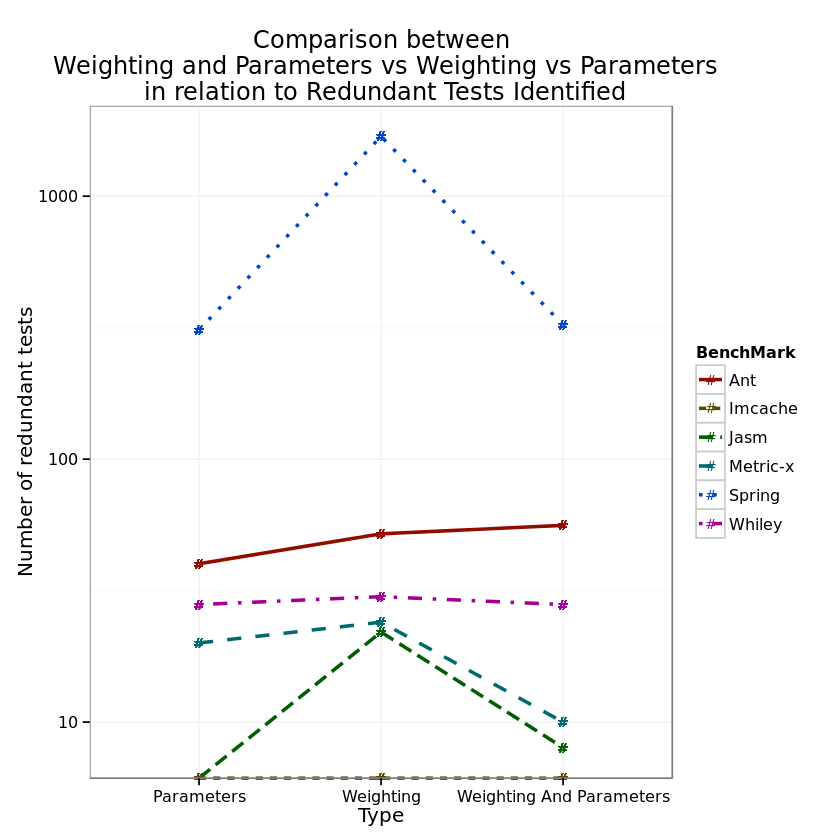
\includegraphics[height=10cm, width = 14.5cm]{WeightNParamVAll.png}
\end{center}
\caption{A figure showing the effect that using weighting and parameters has on the number of redundant tests are identified.}
\label{fig:weightingparamgraph}
\end{figure}

\subsection{Discussion}
Using parameters to increase the confidence\DIFaddbegin \DIFadd{, }\DIFaddend and weighting to remove common method executions should increase the precision of the framework. To appraise the combination, Figure \ref{fig:weightingparamgraph} displays the comparison between each of the three \DIFdelbegin \DIFdel{types}\DIFdelend \DIFaddbegin \DIFadd{techniques}\DIFaddend . Weighting identified more redundant tests in every benchmark \DIFdelbegin \DIFdel{but }\DIFdelend \DIFaddbegin \DIFadd{except }\DIFaddend Ant. Parameters produce similar results to the combination, apart from in Jasm and Metric-x. Whiley coding in Table \ref{whileycoding} show no difference between parameters and the combination. Metric-x's coding Table \ref{metriccoding} hints that the combination may have some appeal by removing all eight limited redundancy tests. At the same time, the similar tests are also removed which is a negative outcome. This suggests that the combination improves the precision for some benchmarks, but not for others. This conclusion means hypothesis 8 can not be accepted. 

Combining weighting and parameters presents interesting time taken results. Table \ref{weightingparamsig} shows that it is nearly identical to the parameters significance table with the only exception being that the Imcache benchmark changed from significant increase in time to a significant decrease in time. This indicates that parameters have a stronger effect than weighting on the final outcome. This is an unexpected result. As previously discussed in Section \ref{sec:param}, one of the reasons that parameters increase the time taken is due to the similar setup and tear down method calls. With weighting removing a large portion of the common method executions it would be expected to cause a decrease in the number of comparisons using parameters. Looking at Appendix \ref{fig:weightparamvparamtime}, this appears to be true for Jasm, Metric-x, Spring and Imcache. However, for Whiley and Ant benchmarks the time to calculate the weighting information is taking longer than the comparisons saved. 

\section{Redundant Test Case Coding}

\begin{table}[h]
\centering

\begin{tabular}{|l|l|l|l|l|}
\hline
                          & \multicolumn{4}{c|}{{\bf Whiley}}                                                             \\ \hline
{\bf Types of redundancy} & \multicolumn{1}{c|}{{\bf Pipeline 2}} & {\bf Weighting} & {\bf Parameters} & {\bf Parameters and Weighting} \\ \hline
Different Equation Value  & 6                                     & 6               & 6                & 6                \\ \hline
Different Equation Sign   & 8                                     & 8               & 8                & 8                \\ \hline
Different Array Values    & 2                                     & 2               & 0                & 0                \\ \hline
Same                      & 10                                    & 10              & 10               & 10               \\ \hline
Limited Redundancy        & 2                                     & 0               & 0                & 0                \\ \hline
Rearranged Equation       & 2                                     & 2               & 2                & 2                \\ \hline
Extra if statement        & 2                                     & 2               & 2                & 2                \\ \hline
                          &                                       &                 &                  &                  \\ \hline
{\bf Total}               & 32                                    & 30              & 28               & 28               \\ \hline
\end{tabular}
\caption{A table displaying a list of coding's for the Whiley Benchmark for four of the different techniques used.}
\label{whileycoding}
\end{table}


\begin{table}[]
\centering
\begin{tabular}{|l|l|l|l|l|}
\hline
                             & \multicolumn{4}{c|}{\textbf{Metric-X}}                                                              \\ \hline
\textbf{Types of redundancy} & \textbf{Pipeline 2} & \textbf{Weighting} & \textbf{Parameters} & \textbf{Parameters  And Weighting} \\ \hline
Different Parameter Value    & 52                  & 10                 & 8                   & 4                                  \\ \hline
Different Object Type        & 6                   & 2                  & 2                   & 0                                  \\ \hline
Different Array Values       & 8                   & 6                  & 4                   & 6                                  \\ \hline
Similar                      & 2                   & 2                  & 0                   & 0                                  \\ \hline
Limited Redundancy           & 8                   & 4                  & 6                   & 0                                  \\ \hline
\textbf{}                    &                     &                    &                     &                                    \\ \hline
\textbf{Total}               & 76                  & 24                 & 20                  & 10                                 \\ \hline
\end{tabular}
\caption{A table displaying a list of coding's for the Whiley Benchmark for four of the different techniques used.}
\label{metriccoding}
\end{table}
 \newpage 
 \newpage \chapter{Conclusions and Future Work}\label{C:future}

\section{Future Work}
\todo{It may be that a lot of tests subsume another rather than are redundant.}
The project has explored the use of higher level information than previously explored for identifying redundant test cases while examining how pre processing and changing the depth of information retrieved can impact the results. Although the output of the framework is adequate in the sense that there is a low number of tests identified, where the developers can easily look over and remove them as they see fit. As discussed in Section \ref{sec:crit} one of the limitations is identifying when one test subsumes another. Using a statement coverage information with weighting would provide an interesting set of results. It would allow for several questions to be answered in regard to the performance of method execution vs statement information. The results would be expected to build off those achieved in Maurer et al. \cite{li2008static}  and Robinson et al. \cite{koochakzadeh2009test}. 

One of the issues identified in Section \ref{sec:pipelineEva}, there was difficult identifying the best pipeline variables to use. In Section \todo{TODO} there are guidelines that are produced which were created based on the benchmarks size and types, although this would highly likely to not be universal. \todo{Finish if I produce guidelines.}

Memory consumption hampered the number of test's that could be run for some of the benchmarks. To overcome this the use of a database could be employed. This would increase the time taken as it would be retrieving the data from non-volatile memory store, but would allow for an increased set of data to be examined, potentially using statement information and method execution data where the method execution data is used during the n-1 pipeline stages and the statement information is explored once the number of potential redundant tests is reduced. \todo{I feel this should be switched around. Combining the statement and method execution should start then why and how.}
\\
\todo{Database usage}\\


\section{Conclusions}

\todo{The use of method execution data seemed like a good candidate to identify matching tests} \\
\todo{Weighting and parameters show potential in helping to limit the number of redundant test cases} \\
\todo{Calling tree has limited effect beyond depth of 1 when by itself}
\todo{Pipelining saved substantial time}

\todo{Talk about framework}
\todo{Talk about strategies}

\begin{itemize}
\item{Explore the use of method execution details}
\item{The impact of weighting on performance}
\item{The impact of parameters on performance}
\item{The impact of calling context depth on performance}
\item{The impact of pipelining the data on performance}
\end{itemize}

\subsection{Can method execution details give a good overview of the level of test redundancy?}

It is difficult to make a direct comparison between using statement information and higher level method execution details without implementing and comparing both on the same benchmarks. Therefore, the level of redundancy identified will be evaluated by the potential redundancy identified as well as the type of redundancies. It is important to take into consideration both. Knowing the number of tests allows us to see how method executions handle different types of tests, unit vs end to end respectively. The potential redundancy gives us insight into the types of redundant tests identified, giving information on which types of test redundancy is easier to pick up and which is harder when using method execution.

The use of method execution allows us to look at test cases that produce a larger amount of total information, in particular ones which are end to end tests (Whiley) which produce a large amount of data. It would be interesting to see the comparison between statement information and method execution details. It appears to be intuitive that statement coverage would give more accuracy in regard to determining whether two test cases are redundant but this would come at a cost of time and memory consumption. What is the optimal trade-off for this situation? \todo{Maybe talk about it here?}

By using a higher abstraction of information, there appears to be no relation to the time taken and the number of redundant test cases with the two types of test cases, unit and end to end respectively.

Examining the Table \ref{whileycoding} and \ref{metriccoding}, allows for an comparison to identify the difference between end to end tests and unit tests while using method execution details. It appears that the types of the tests may react differently to the settings used. For the end to end test of Whiley, where the size of a single test case is larger than Metric-x, it appears to respond to the use of parameters and weighting in a positive manner. Where the tests that are picked up as limited redundancy by the Pipeline 2 are both removed when weighting and parameters are used. In comparison to the unit test case. The unit test appeared to not respond either to weighting or parameters by identifying tests that had limited redundancy. When combining both of these, it removed the tests that were identified, but had limited redundancy. \todo{Explain why it might be happening} This may reflect on the amount of pre processing and information needed for the different types to get identified. \todo{This would mean that the larger bench marks can be analysed faster ?}


\subsection{Can we improve the overall performance with weighting?}
\todo{More}
Weighting attempts to improve the accuracy of the redundancy by removing false-positives while improving the time taken to analyse. 

\todo{Examine the coding tables, state that using weighting can help}

\subsection{Can we improve the performance using parameters?}

The answer to the question depends on the type of parameters that are used. Initially the only parameters that were being retrieved were the primitive types. The reason was due to the easy nature of retrieving the values of them. This lead to a less than expected outcome as the majority of parameters involved object types which contained the important information that could be used to increase the separability of tests. By using reflection to retrieve the fields of these objects allowed more insight into the content that the parameter objects were holding and the nature of them, but it also meant more data had to be held and analysed resulting in an increased time taken. There exists this trade off between time taken and confidence of redundancy when using parameters. The reason for running a framework such as this is to reduce the number of redundant test cases, therefore the majority of situations will prefer a higher confidence of redundancy over time taken. The answer is then to use reflection to retrieve the parameters.

Examining the weighting and parameter time taken in Appendix \ref{fig:weightparamtime}, it shows that when weighting is taken into account with parameters then for Jasm, the time taken goes from just under five minutes to just under one minute.

\todo{Examine the coding tables, state that using parameters improves performance}

\subsection{Can Calling Trees we used to better identify redundant tests?}

The result was unexpected. It showed that as the depth of the calling context increased, there was limited level of reduction in the number of redundant tests identified. Although there was a change, it was lower that what was expected. A possible reason for this was after a certain number of calling context, the tests that were going to be different, were already different and increasing the size of the calling tree did not affect it. This may imply that using a calling context depth of two is enough to generate a list of redundant tests similar to a depth of two. \todo{Todo check with K Length Comparison - might be talking about same things}

Using a calling tree allows for the analysing tool to better identify redundant tests as shown by the comparison above where the one, two and three calling sizes are compared.

\subsection{How does pipelining impact the time taken?}

Pipelining was one of the critical aspects of the project. It not only lead to a decrease in the time taken but also the memory consumed. Like calling trees, there is an optimal number of pipelines before they are causing a larger increase in time than they save. We can see in the results that each \todo{check results} benchmark responded differently to the length of the pipeline. This may have been due to not finding the optimal pipeline variables for the second pipeline causing a large number of comparisons still being needed to be done by the last pipeline. Another reasons may have been due to the nature of the tests where they were difficult to separate until you used more data such as a list or calling context. 

\todo{Maybe guidelines for the settings that each type of test should use?}

\section{Justify your approach}

\todo{Unsure if I should put anything ehre}


\section{Critically evaluate your study}
\label{sec:crit}
A major limitation to the study was volatile memory. For test suites such as Whiley, storing the parameter data and calling context endured a high level of volatile memory usage, limiting the amount of tests for Whiley that were able to be retrieved (Limited to valid tests). An approach that should have been considered with more thought was the use of a database. Although this would have introduced difficulty reducing the non-deterministic behaviour to a minimum. A major factor would be the difficulty around executing the analysis on a grid system and replicating the conditions each run.

Some of the benchmarks that were chosen contain multiple unit tests within one test case. The framework described throughout this paper would not be able to pick up when a test case subsumes another. The frame work only looks at the total method set, and for each of the singular unit tests, there would need to be a skewed proportion of the conjoined test case in regard to the total method executions. This means that unless one of the unit tests within the conjoined test case was arbitrary larger than the other, roughly 98:1 lines of code then it would not be picked up as being redundant, unless there was another conjoined test case similar. This is where the other approaches identified in Chapter \ref{C:related} would be more effective. By looking at the statement information, it is easier to determine when a test is a subset of another and have more confidence on it being a redundant test case in comparison to looking at solely the method execution details. \todo{Need to explain this better.}

As discussed in Section \ref{sec:pipelineEva}, some benchmarks performed better with a two stage pipeline in comparison to a three stage, and vice versa. This may have been due to not being able to identify the optimal parameters for each benchmark, although there were multiple different parameters tested to explore each benchmark's optimal. \todo{Maybe explore how I decided the optimal ?} \newpage 
 \newpage \begin{appendices}
\chapter{The effect of pipeline size in regard to the time taken}
\begin{figure}[h]
\centering
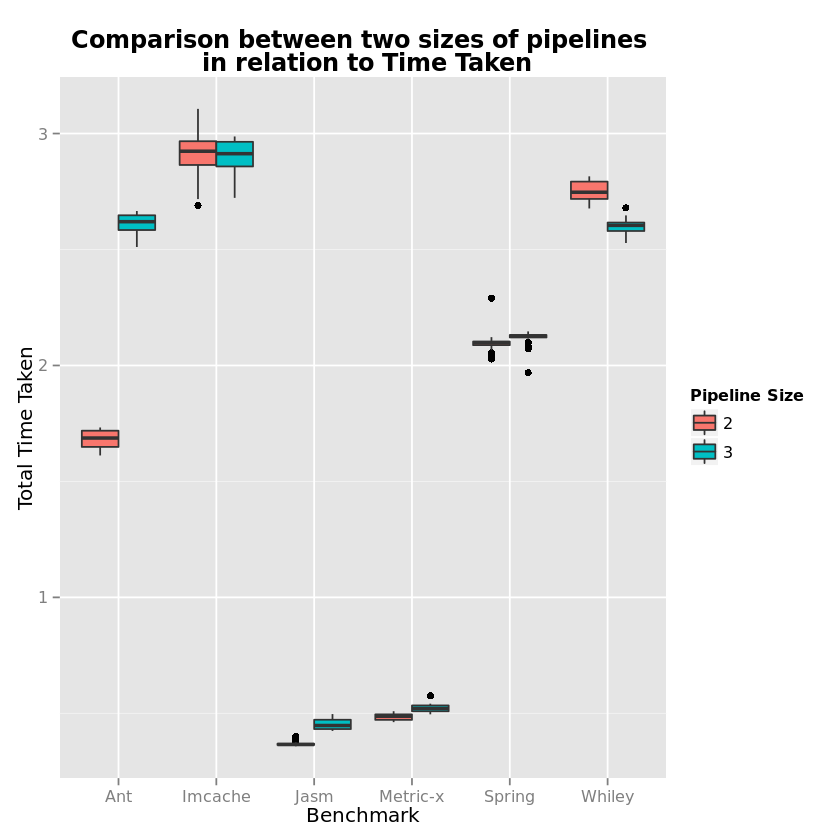
\includegraphics[width=\textwidth,height=13cm]{PipelineTime.png}
\caption{A figure showing the relationship that using different pipeline sizes has on the total time taken to analyse the data.}
\label{fig:pipelinetime}
\DIFdelbeginFL %DIFDELCMD < \end{figure}
%DIFDELCMD < 

%DIFDELCMD < %%%
\chapter{\DIFdelFL{Pipeline linear scaling}}
%DIFAUXCMD
\addtocounter{chapter}{-1}%DIFAUXCMD
%DIFDELCMD < \begin{figure}[h]
%DIFDELCMD < \centering
%DIFDELCMD < 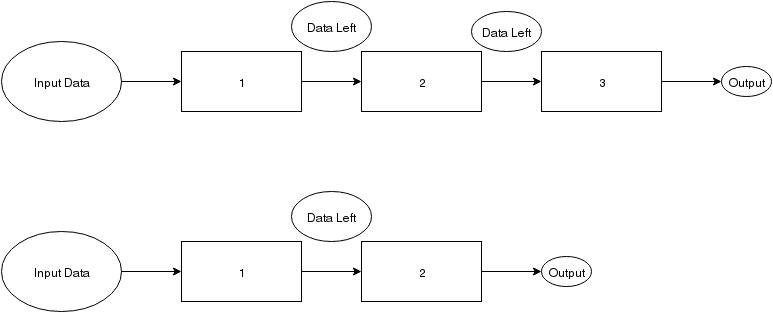
\includegraphics[width=\textwidth,height=10cm]{PipelineComp.png}
%DIFDELCMD < %%%
%DIFDELCMD < \caption{%
{%DIFAUXCMD
\DIFdelFL{The circle size represents the data that is left in the pipeline. The figure shows that the difference that is between a two stage pipeline and a three stage only has limited room for a reduction in test cases identified. This shows that the time taken to run the extra pipeline costs more than it saves.}}
%DIFAUXCMD
%DIFDELCMD < \label{fig:pipelinecomp}
%DIFDELCMD < %%%
\DIFdelendFL \end{figure}

\chapter{The effect of K Depth in regard to the time taken}
\begin{figure}[h]
\centering
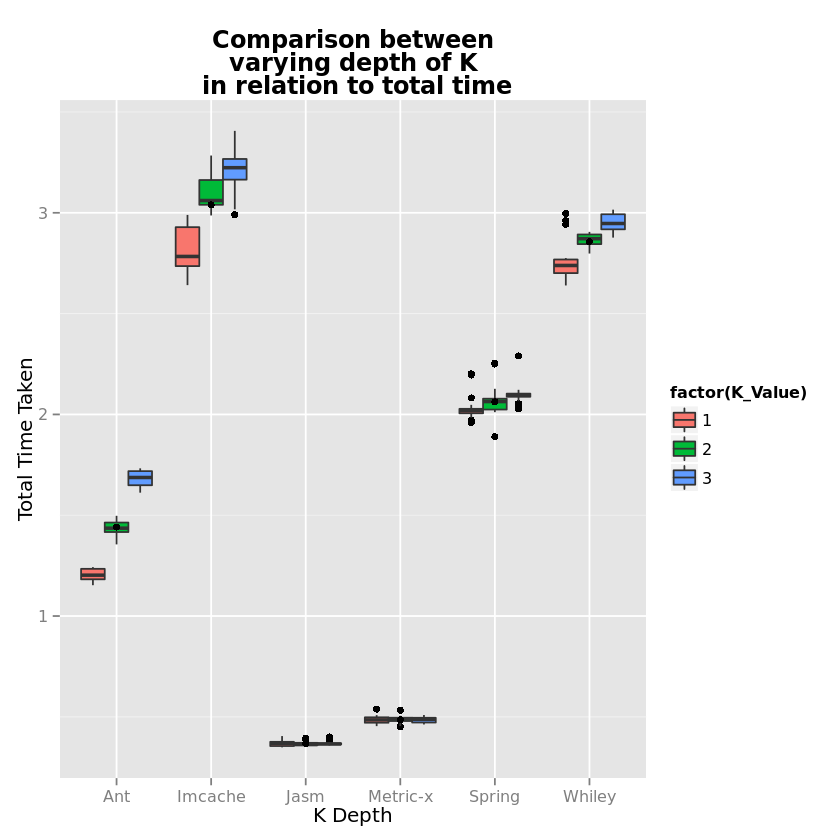
\includegraphics[width=\textwidth,height=13cm]{KDepthTime.png}
\caption{A figure showing the relationship that using a different K Depth has on the total time taken to analyse the data.}
\label{fig:kdepthtime}
\end{figure}

\chapter{The effect of parameters in regard to the time taken}
\begin{figure}[h]
\centering
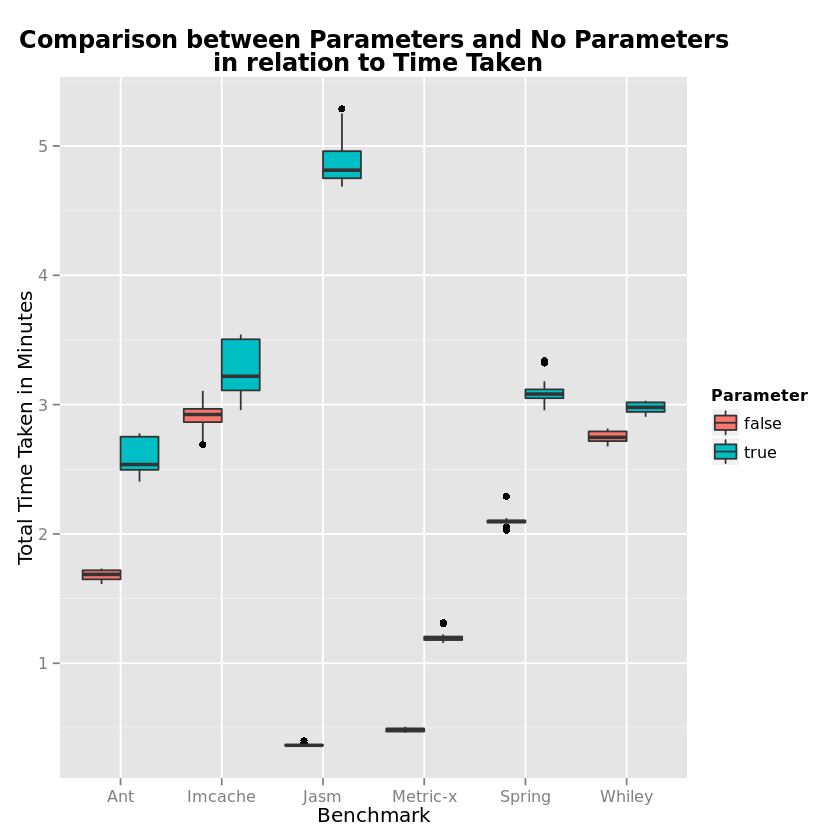
\includegraphics[width=\textwidth,height=13cm]{ParamTime.png}
\caption{A figure showing the relationship that using parameters has on the total time taken to analyse the data.}
\label{fig:paramtime}
\end{figure}

\chapter{The effect of weighting in regard to the time taken}
\begin{figure}[h]
\centering
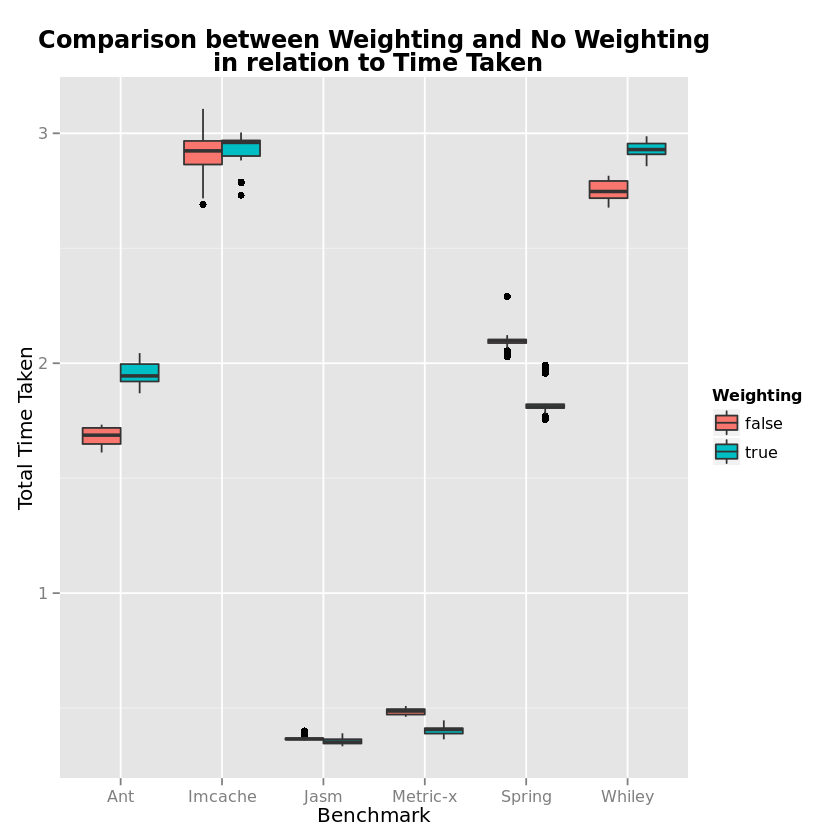
\includegraphics[width=\textwidth,height=13cm]{WeightTime.png}
\caption{A figure showing the relationship that using weighting has on the total time taken to analyse the data.}
\label{fig:weighttime}
\end{figure}

\chapter{The effect of weighting and parameters combined in regard to the time taken}
\begin{figure}[h]
\centering
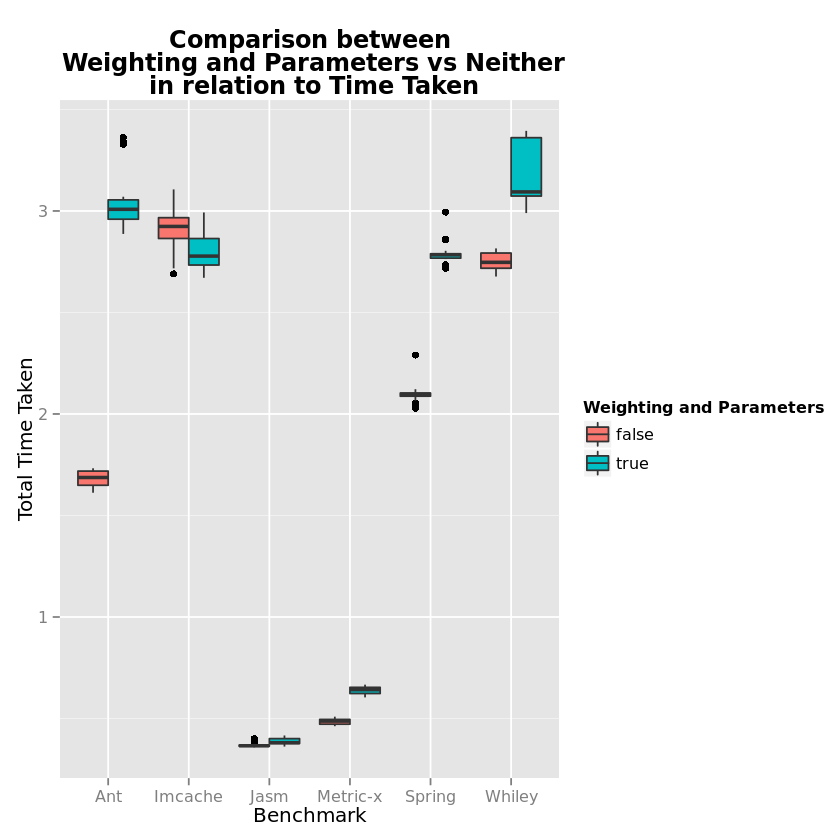
\includegraphics[width=\textwidth,height=13cm]{WeightnParamTime.png}
\caption{A figure showing the relationship that using weighting and parameters combined has on the total time taken to analyse the data.}
\label{fig:weightparamtime}
\end{figure}

\chapter{The effect of weighting and parameters vs parameters in regard to the time taken}
\begin{figure}[h]
\centering
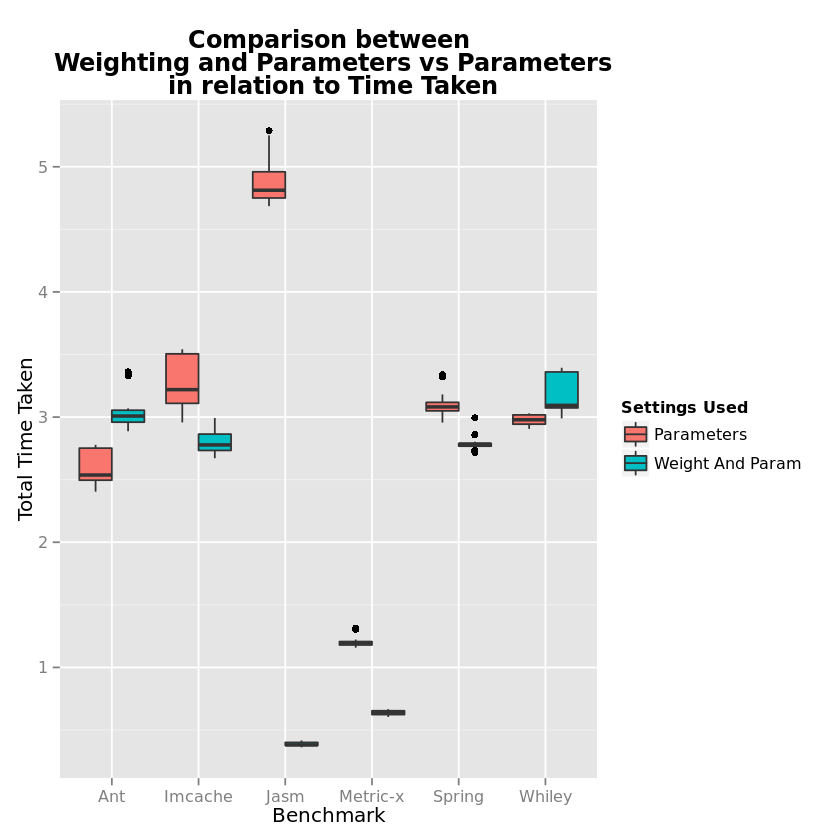
\includegraphics[width=\textwidth,height=13cm]{WeightnParamvParamTime.png}
\caption{A figure showing the relationship that using weighting and parameters combined vs parameters alone has on the total time taken to analyse the data.}
\label{fig:weightparamvparamtime}
\end{figure}




\end{appendices} \newpage 

%%%%%%%%%%%%%%%%%%%%%%%%%%%%%%%%%%%%%%%%%%%%%%%%%%%%%%%

\backmatter

%%%%%%%%%%%%%%%%%%%%%%%%%%%%%%%%%%%%%%%%%%%%%%%%%%%%%%%


%\bibliographystyle{ieeetr}
\bibliographystyle{acm}
\bibliography{sample.bib}


\end{document}
